% This is "sig-alternate.tex" V2.0 May 2012
% This file should be compiled with V2.5 of "sig-alternate.cls" May 2012
%
% This example file demonstrates the use of the 'sig-alternate.cls'
% V2.5 LaTeX2e document class file. It is for those submitting
% articles to ACM Conference Proceedings WHO DO NOT WISH TO
% STRICTLY ADHERE TO THE SIGS (PUBS-BOARD-ENDORSED) STYLE.
% The 'sig-alternate.cls' file will produce a similar-looking,
% albeit, 'tighter' paper resulting in, invariably, fewer pages.
%
% ----------------------------------------------------------------------------------------------------------------
% This .tex file (and associated .cls V2.5) produces:
%       1) The Permission Statement
%       2) The Conference (location) Info information
%       3) The Copyright Line with ACM data
%       4) NO page numbers
%
% as against the acm_proc_article-sp.cls file which
% DOES NOT produce 1) thru' 3) above.
%
% Using 'sig-alternate.cls' you have control, however, from within
% the source .tex file, over both the CopyrightYear
% (defaulted to 200X) and the ACM Copyright Data
% (defaulted to X-XXXXX-XX-X/XX/XX).
% e.g.
% \CopyrightYear{2007} will cause 2007 to appear in the copyright line.
% \crdata{0-12345-67-8/90/12} will cause 0-12345-67-8/90/12 to appear in the copyright line.
%
% ---------------------------------------------------------------------------------------------------------------
% This .tex source is an example which *does* use
% the .bib file (from which the .bbl file % is produced).
% REMEMBER HOWEVER: After having produced the .bbl file,
% and prior to final submission, you *NEED* to 'insert'
% your .bbl file into your source .tex file so as to provide
% ONE 'self-contained' source file.
%
% ================= IF YOU HAVE QUESTIONS =======================
% Questions regarding the SIGS styles, SIGS policies and
% procedures, Conferences etc. should be sent to
% Adrienne Griscti (griscti@acm.org)
%
% Technical questions _only_ to
% Gerald Murray (murray@hq.acm.org)
% ===============================================================
%
% For tracking purposes - this is V2.0 - May 2012

\documentclass{sig-alternate}

\usepackage{multirow}
\usepackage{graphicx}
\usepackage{algorithm}
\usepackage{algorithmic}
\usepackage{color}
\usepackage{caption}
\DeclareCaptionType{copyrightbox}
\usepackage{subcaption}
\usepackage{mdwlist}
\newtheorem{definition}{Definition}
\usepackage{amsmath}
\usepackage{url}
\usepackage{algorithm}
\usepackage{algorithmic}
\usepackage{booktabs}
\usepackage{amssymb}
\renewcommand{\algorithmicrequire}{\textbf{Input:}}
\renewcommand{\algorithmicensure}{\textbf{Output:}}
\newcommand{\todo}[1]{{\textcolor{red}{{\bf TODO:} #1}}}
\newcommand{\tabincell}[2]{\begin{tabular}{@{}#1@{}}#2\end{tabular}}
\usepackage{threeparttable}

\begin{document}
%
% --- Author Metadata here ---
\conferenceinfo{WOODSTOCK}{'97 El Paso, Texas USA}
%\CopyrightYear{2007} % Allows default copyright year (20XX) to be over-ridden - IF NEED BE.
%\crdata{0-12345-67-8/90/01}  % Allows default copyright data (0-89791-88-6/97/05) to be over-ridden - IF NEED BE.
% --- End of Author Metadata ---

\title{Information-theoretic Detection of Non-Redundant Overlapping Communities in Attributed Graphs}
%\subtitle{[Extended Abstract]
%\titlenote{A full version of this paper is available as
%\textit{Author's Guide to Preparing ACM SIG Proceedings Using
%\LaTeX$2_\epsilon$\ and BibTeX} at
%\texttt{www.acm.org/eaddress.htm}}}
%
% You need the command \numberofauthors to handle the 'placement
% and alignment' of the authors beneath the title.
%
% For aesthetic reasons, we recommend 'three authors at a time'
% i.e. three 'name/affiliation blocks' be placed beneath the title.
%
% NOTE: You are NOT restricted in how many 'rows' of
% "name/affiliations" may appear. We just ask that you restrict
% the number of 'columns' to three.
%
% Because of the available 'opening page real-estate'
% we ask you to refrain from putting more than six authors
% (two rows with three columns) beneath the article title.
% More than six makes the first-page appear very cluttered indeed.
%
% Use the \alignauthor commands to handle the names
% and affiliations for an 'aesthetic maximum' of six authors.
% Add names, affiliations, addresses for
% the seventh etc. author(s) as the argument for the
% \additionalauthors command.
% These 'additional authors' will be output/set for you
% without further effort on your part as the last section in
% the body of your article BEFORE References or any Appendices.

\numberofauthors{1} %  in this sample file, there are a *total*
% of EIGHT authors. SIX appear on the 'first-page' (for formatting
% reasons) and the remaining two appear in the \additionalauthors section.
%
\author{
% You can go ahead and credit any number of authors here,
% e.g. one 'row of three' or two rows (consisting of one row of three
% and a second row of one, two or three).
%
% The command \alignauthor (no curly braces needed) should
% precede each author name, affiliation/snail-mail address and
% e-mail address. Additionally, tag each line of
% affiliation/address with \affaddr, and tag the
% e-mail address with \email.
%
% 1st. author
\alignauthor
Jing Feng \hspace{12 mm} Nina Hubig \hspace{12 mm} Xiao He \hspace{12 mm} Claudia Plant\\
	   \affaddr{integrative Knowledge Discovery in Databases Group}\\
       \affaddr{University of Munich, Helmholtz Zentrum M\"unchen, Technische Universit\"at M\"unchen }\\
       %\affaddr{integrative Knowledge Discovery in Databases Group}\\
      % \affaddr{Wallamaloo, New Zealand}\\
       \email{\{feng,he\}@dbs.ifi.lmu.de, \{nina.hubig, claudia.plant\}@helmholtz-muenchen.de}
% 2nd. author
%\alignauthor
%Nina Hubig\\
%       \affaddr{Helmholtz Zentrum M\"unchen, Technische Universit\"at M\"unchen}\\
%      % \affaddr{P.O. Box 1212}\\
%       %\affaddr{Dublin, Ohio 43017-6221}\\
%       \email{nina.hubig@helmholtz-muenchen.de}
%\and
%% 3rd. author
%\alignauthor
%Xiao He\\
%       \affaddr{University of Munich}\\
%      % \affaddr{1 Th{\o}rv{\"a}ld Circle}\\
%      % \affaddr{Hekla, Iceland}\\
%       \email{he@dbs.ifi.lmu.de}
%%\and  % use '\and' if you need 'another row' of author names
%% 4th. author
%\alignauthor 
%%Christian B\"ohm\\
%%       \affaddr{University of Munich}\\
%%      % \affaddr{Brookhaven National Lab}\\
%%       %\affaddr{P.O. Box 5000}\\
%%       \email{boehm@dbs.ifi.lmu.de}
%% 5th. author
%\alignauthor Claudia Plant\\
%       \affaddr{Helmholtz Zentrum M\"unchen, Technische Universit\"at M\"unchen}\\
%      % \affaddr{Moffett Field}\\
%       %\affaddr{California 94035}\\
%       \email{claudia.plant@helmholtz-muenchen.de}
}
% There's nothing stopping you putting the seventh, eighth, etc.
% author on the opening page (as the 'third row') but we ask,
% for aesthetic reasons that you place these 'additional authors'
% in the \additional authors block, viz.
%\additionalauthors{Additional authors: John Smith (The Th{\o}rv{\"a}ld Group,
%email: {\texttt{jsmith@affiliation.org}}) and Julius P.~Kumquat
%(The Kumquat Consortium, email: {\texttt{jpkumquat@consortium.net}}).}
%\date{30 July 1999}
% Just remember to make sure that the TOTAL number of authors
% is the number that will appear on the first page PLUS the
% number that will appear in the \additionalauthors section.

\maketitle

\begin{abstract}
How to mine complex and useful knowledge from an attributed graph? For many real world data, consider e.g. social networks, we do not only have a graph representing e.g. the friendship network, but also a lot of additional attributes further characterizing the nodes, e.g. information on hobbies, gender, location, etc. Some techniques for clustering such complex data have recently been proposed. However, existing algorithms suffer the drawbacks that they either require many input parameters which are difficult to estimate, or they only recognize the overlap in the graph structure or in the attributes of the nodes but not in both. With overlap we mean that nodes as well as attributes might be assigned to multiple different clusters.
Avoiding overlap implies  losing information. For that reason we propose a method that enables combined overlap in both the underlying network structure and the attribute subspaces of each node. But allowing that much overlap raises another challenge: How to handle redundancy? 
As solution this paper proposes a non-redundant method called IROC (for \emph{I}nformation-theoretic non-\emph{R}edundant \emph{O}verlapping \emph{C}lustering) that evaluates complex attributed graphs in an  automatic way. We are the first that emphasize the importance of mining overlapping communities in all aspects of an attributed graph. Our experiments show that IROC reveals meaningful information in both real world - and synthetic data sets.

\end{abstract}

% A category with the (minimum) three required fields
%\category{H.4}{Information Systems Applications}{Miscellaneous}
%A category including the fourth, optional field follows...
%\category{D.2.8}{Database Management}{Database Applications}[Graph Mining]

%\terms{Algorithms}

\keywords{graph mining, social networks, attributed graph,} %  non-redundant, overlapping, parameter-free

\begin{figure}[h]
\centering
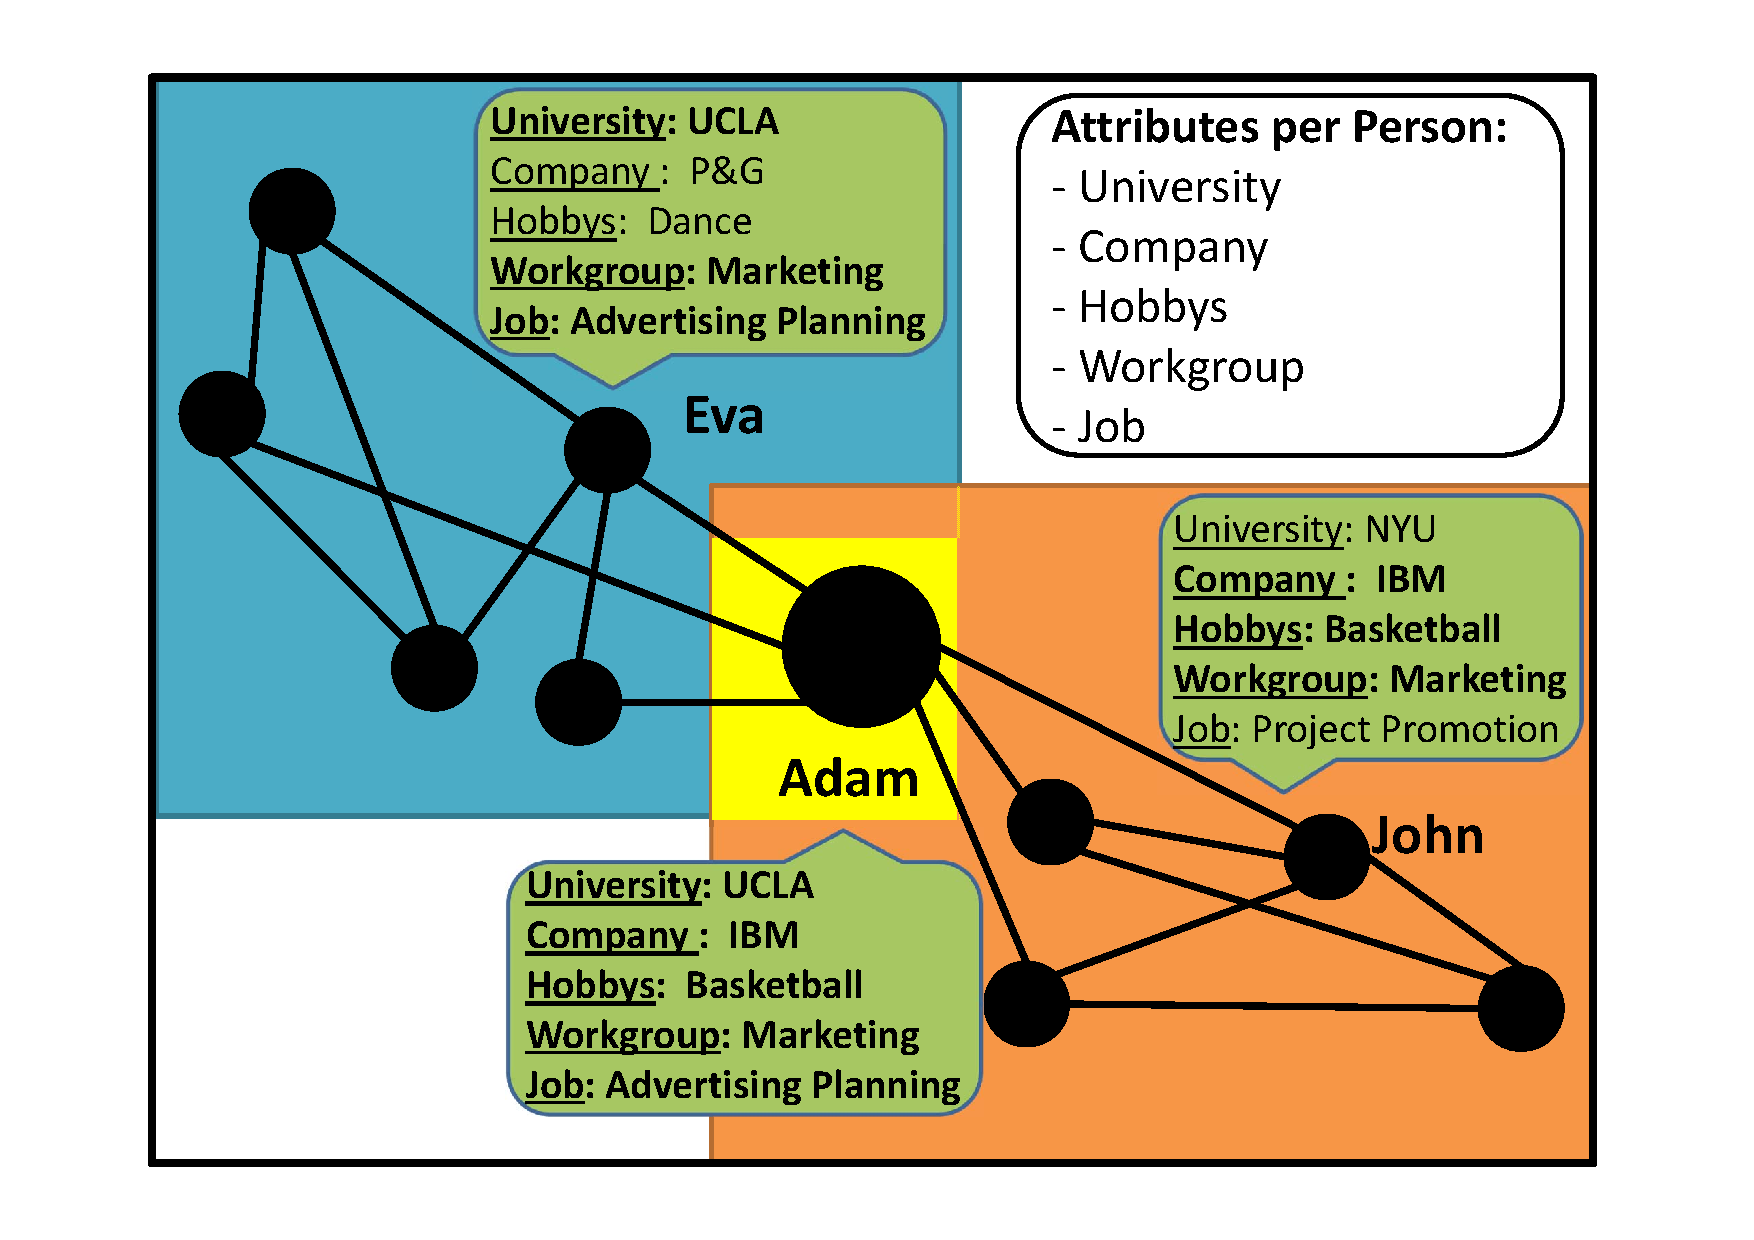
\includegraphics[width = 0.8\columnwidth]{figure/example.pdf}
\caption{Motivational example of a social friendship network.}
\label{fig:a}
\end{figure}

\section{Introduction}
Social networks, gene-and/or protein interaction networks as well as nearly all common types of networks in real world applications are not only sharing a large amount of information depending on the relationship between the vertices, but also contribute information regarding the characteristics of these vertices. These characteristics are modeled as attributes of a graphs' vertex. Thus we are referring to a graph containing extra information in its nodes as an \emph{attributed graph}. These attributed graphs connect two aspects of information: First, the structural "who knows whom" connection given by the graph itself as for example in friendship relationships of applications like facebook. Second, the attributes per node or person showing (in the case of facebook) personal ego-information like hobbys, what they are working, where they are living etc. Combining both aspects of information gives the chance to analyze things like "what has this friendship circle in common" or "what do most people in my work environment like and what joins them together?". Questions like this can be answered to some extend by just clustering attributed graphs, as existing algorithms propose in \cite{DBLP:conf/icdm/ZhouCY10}, \cite{DBLP:conf/sigmod/XuKWCC12} and \cite{DBLP:journals/pvldb/ZhouCY09}. But we are not only clustering attributed graphs but are also applying an overlapping concept to both informational aspects - to the graph structure and to the attribute space. What do we mean by overlapping and what do we gain out of the attributed graph if we are already able to group both informational aspects by just partitioning the attributed graph?


% what exactly does overlapping mean?

%Consider the fun example given in  Fig.\ref{fig:a} to outline the meaning of "overlapping" in combination with attributed graphs. It shows the friendship circle of a person called "Adam", he connects to people from his work environment and to people from outside his work environment that are still more or less living nearby like in the same city. The distance of the city-nodes to Adam visualizes how close they live together. Every person has the attributes of where he lives in, where he works and what hobbys he or she has. You could also think of the hobbys as more of a list, containing several attributes and differing in detail. Our Adam is living in detail in Vancouver, works at Eden Garden Center and likes skydiving as a hobby. The overlapping of the at least three dimensional attribute space and its corresponding friendship links is visualized in colored rectangles behind the graph structure. People in the same work environment likely know each other more than people from just the same city. We take a look at the two named nodes Lillith and Eva. Lillith is a working partner of Adam, living in the same city who shares some hobbys with him, lets say they even share skydiving. Let Eva be Adams' girlfriend living also close to Adam and sharing some interests, but not necessarily working together. Now, how would an attributed graph partitioner most likely divide this structure if no overlap is allowed? A possibility would be that Lillith is grouped together with the other working partners of Adam, creating a nearly full clique and therefore high quality in terms of clustering. Her share of hobbys with Adam and even Eva might be lost. With overlapping, Lillith being present in several communities would not only be in the one with the working people but also in a subspace cluster containing all people with similar hobbys (and living nearby) like Eva and Adam. She is also present in a very small connected group but highest dimensional attribute space in terms of all people that work together and have similar hobbys consisting only of Lillith and Adam. All in all this small example already shows the range of interpretability and complexity reduced from real world data when overlapping is not integrated.

Consider the example given in Fig.\ref{fig:a}, it outlines the meaning of ``overlapping" in combination with an attributed graph. The figure shows the friendship circles in a social network of a person called ``Adam". 
%He connects to people from the company he has worked in and to people who has studied in the same university with him. 
His two friendship circles are visualized in colored rectangles behind the graph structure: blue stands for his friends from school and orange indicates his circle of colleagues. The overlapping of both circles is highlighted in yellow. Every person (node) includes attributes on their university,  their working place and department, what hobbies they have and what job position they are in. % or she has studied, which company he or she works for, what hobbies he or she has, which department he or she works in and what type of job he or she does. 
You could also think of these attributes as more of a list, containing several items and differing in detail.
For example, Adam graduated from UCLA, works in IBM, likes playing basketball, works in the marketing department and is mainly in charge of planning advertisements. Now, how would an attributed graph partitioner most likely divide this structure if no overlap is allowed? A distinct possibility is to assign Adam to either the blue or the orange circle, because Adam can form a nearly full clique with both circles. This would result in a very high quality for clustering for one cluster while the other would lose some information (Adam). In this frequent case, partitioning must sacrifice the quality of this one cluster. Obviously, overlapping clustering, like assigning Adam to both circles, provides more meaningful structural information. Lets take a look at the two named nodes John and Eva that share some overlap in their attributes with Adam. John is a working partner of Adam, and shares the same hobby, workgroup and of course company with him. Also Eva graduated from the same university, shares the same workgroup and is working in a similar job like Adam, just in a different company. Therefore, Adam shares similar subspace attributes with his work circle where John is, while he shares other subspace with his school circle where Eva is. Apparently Adam should be assigned to both circles from the attribute information side as well.
%Besides, both John and Eva overlap with Adam on their workgroup, thus indicating the overlap different friendship clusters may representing a small connected cluster even though they are present in different friendship circles. Partitioning the graph structure would never reveal this small cluster. 
All in all this small example already shows the range of interpret-ability and complexity reduced from real world data when overlapping is not integrated.

%And he would not only be in the one with the people working in same workgroup of same company and even with same hobby, but also be a member of the one with people studying in same university and engaging in same job in same type of workgroup. Thus, overlapping (``Workgroup") also exists among detected coherent attributes which convey the meaning of the cluster.  

Therefore, we contribute a new method of clustering attributed graphs with the objective to find the reasonable overlapping communities and meaningful subspace of the attributes at the same time based on an information theoretical technique. The advantages of the proposed algorithm are in short:

\begin{itemize}
\item  \textbf{Discovery of overlapping communities}:
Our meth\\-od discovers not only single dense groups of friends but also their connections to other groups. Node structures can have several group memberships and be efficiently evaluated.
\item  \textbf{Finding coherent attribute subspaces}:
We think that some information is hidden in attribute subspaces that can be obtained to express the meaning of the cluster. Overlapping is also allowed among attribute subspaces.  
\item  \textbf{Without Redundancy}: 
Based on the Minimum Description Length (MDL) principle \cite{mdlbook}, our approach balances quality and redundancy in both graph structure and attribute space. Specifically, a node is only assigned to several graph clusters and an attribute is only part of multiple subspaces if this pays-off in terms of data compression. Thereby, only the truly relevant overlap useful to compress the data is reported as a result of our algorithm.
\item  \textbf{Automation}:
Our information theoretic based algorithm relieves the user from the task of finding parameters to run the method on every specific data. The non-redundant overlapping clusters and coherent attribute subspace can be detected automatically.  
%Basically we only need to retrieve one parameter specifically from the data, this parameter is of course evaluated in the experiments section, to show its very robust and thus it is possible to be chosen automatically.
\end{itemize}

The remainder of this paper is organized as follows: In the following section, we elaborate our coding scheme, which is necessary to avoid parametrization and balances among quality and redundancy. Section 3 describes the algorithm in detail. Section 4 shows experiments and results. Related work is discussed in Section 5. The conclusion follows in Section 6.

%With increasing complexity of data, graph has not sticked to only convey structural relation between vertices. A vertex if considered as an independent object contains information describing its character. For example,   Community detection is a significant task in mining graph data. Transitionally,  However, attributes plays a pivotal role in discovering knowledge from data as well. With the assistant of node attributes, more
% data element is able to possess multiple intimate connections to other data elements especially for graph data.  Therefore, overlapping exists between communities.
%
%In this paper, we proposed an information theoretic based algorithm which not only detects communities of an attributed graph with overlapping vertices but also discovers coherent subspace of attributes. The mainly contributions of our algorithm is conveyed as follow.
%
%1. Overlapping community detection:
%
%
%2. Finding coherent attributes subspace


\section{Compressing an Attributed Graph}
%\begin{table}[h]
%\center\caption{Table of Symbols and Acronyms.}
%\begin{tabular}{|c|c|}
%\hline
%Symbols & Definitions\\
%\hline\hline
%$MDL$ & Minimum Description Length\\
%$IROC$ & Information-theoretic non-Redundant Overlapping Clustering\\
%\hline
%$G$ & Attributed graph\\
%$V$ & Set of vertices of a graph\\
%$E$ & Set of edges of a graph\\
%$\Lambda$ & Dimension of the attribute space \\
%$\Theta$ & Number of categories \\
%$A$ & Adjacency matrix\\
%$F$ & Attribute matrix (in some literature also called feature matrix)\\
%$C$ & Cluster in the graph\\
%$U$ & No-Cluster area, logically "unclustered"\\
%$N$ & Number of vertices \\
%$K$ & Number of Cluster \\
%$N_C$& Number of vertices in cluster $C$ \\
%$T$ & Number of all attributes, same as $|\lambda|$ for clarity reasons\\
%$\lambda_i$ & The $i$th attribute, $1<i<T$\\
%$\theta_i$ & Categories of $i$th attribute, $1<i<T$\\
%$S$ & Number of attributes of cluster $C$ \\
%$L(D|M)$ & coding costs of data D under model M \\
%$P$ & a probability, we like upper letters \\
%$ID$ & a cluster label (id)\\
%\hline
%\end{tabular}
%\label{tab:symbols}
%\end{table}
To understand our coding scheme it is foremost important to outline what needs to be compressed in an attributed graph. From start, attributed graphs are an extension from general graphs by involving attributed information to each vertex. Therefore, two types of matrices are needed to model both structural connections in the graph and the attribute space of each node. Same as the general graph, the structure is mapped into an adjacency matrix, while the attributes of each vertex can be modelled as a matrix with rows denoting vertices and columns representing attributes.  We call that matrix an \emph{attribute matrix}. So far, an attributed graph is represented by an adjacency matrix and an attributed matrix that need to be compressed for efficiency and automatization. For simplicity in this paper, we focus on undirected unweighed graphs with categorical attributes, which means both matrices are symmetric.

\subsection{Notations}

%\noindent \emph{Attributed graph} is an extension of general graph by involving attributes for each vertex, which combines relational information with descriptive information. Therefore, two matrices are adopted to represent such type of graph. Specifically, like the general graph connections between vertices are mapped as $``1"$s in an adjacency matrix, while the attributes of all vertices can be arrayed into a matrix, which is named as \emph{attribute matrix}, with rows denoting vertices and columns representing various attributes. The two matrices are related by sharing same vertices. An attribute graph $G$ is represented by an adjacency matrix $A$ and an attribute matrix $F$, which is defined in Definition \ref{def:an}. In this paper, we focus on undirected unweighed graphs with categorical attributes. 
Before we start with the coding scheme this section describes the used notation in the paper for clarification.

\begin{definition}[Attributed Graph]\label{def:an}
An attributed g-raph is defined as $G=(V,E,\Lambda)$, where $V = \{v_1, v_2,...,v_N \}$ contains $N$ vertices, $E= \{(v_i,v_j),1\leq i\leq N,1\leq j \leq N,i\neq j \}$ are edges, $\Lambda = \{\lambda_1,\lambda_2,...,\lambda_T \}$ are $T$ attributes of each vertex. $\Theta = \{\theta_1,\theta_2,...,\theta_T \}$ represents domains of $\Lambda$. $A$ is the adjacency matrix with $a_{ij}=1$ if $(v_i,v_j)\in E$ and $F$ is the attribute matrix with $f_{ik}$ denotes the categorical value of the $i$th vertex in the $k$th attribute. An attribute graph is represented as $G=(A,F)$ as well.
\end{definition}

In this paper, we aim at mining knowledge from the attributed graph by detecting non-redundant overlapping clusters. As attributed graphs possess both structural and attribute information, the cluster of such type of data covers both informations as well, which is defined in Definition \ref{def:anclus}. A cluster $C$ is a subset of an attributed graph $G$. Specifically, the cluster not only needs to be densely connected but also contains a subgroup of attributes to describe the meaning of the cluster. 
                                                            
\begin{definition}[Cluster in an Attributed Graph]\label{def:anclus}
A cluster is defined as $C =(V',E',\Lambda')$, which is a subset of the attributed graph $G$, where $V'\subseteq V$, $E'\subseteq E$, $\Lambda'\subseteq \Lambda$. $V' = \{v'_1, v'_2,...,v'_{N'} \}$ is a subset of $V$, which includes $N'$ densely connected vertices and $\Lambda' = \{\lambda'_1,\lambda'_2,...,\lambda'_S \}$ is a subset of $\Lambda$, which contains $S$ attributes with coherent categories, where $S\leq T$. $A_C \subset A$ is the subset adjacency matrix of $C$ that only contains the vertices in $C$ and $F_C \subset F$ is the subset attribute matrix of $C$. Similarly, a Cluster is represented as $C=(A_C,F_C)$.
\end{definition}

Besides the own structure of a cluster, there are some edges connecting these clusters that are not included inside the clustering. Similarly to the edge structure, many attributes from the full-dimensional subspace are not assigned to any cluster. We define these areas as the non-cluster area of an attributed graph in Definition \ref{def:nonclus}, which consists of the elements lying outside any cluster. 
                                 
\begin{definition}[Non-Cluster Area]\label{def:nonclus}
The non-cluster area of an attributed graph $G$ modelled by $K$ clusters $\{C_1$, $C_2,...,C_K \}$ is defined as $U = U_A \bigcup U_F $, where $U_A$ is the Non-Cluster area in the adjacency matrix $A$ and $U_F$ is the non-cluster area in the attributed matrix $F$. $U_A=A\setminus A'$, where $A' = A_{C_1}\cup A_{C_2}...\cup A_{C_K}$ is the combination of all structural elements appearing in $\{C_1,C_2,...,C_K \}$ and $U_F = U_{\lambda_1}\cup U_{\lambda_2}...\cup U_{\lambda_T}$, where $U_{\lambda_t}$ are entries of $F$ in attribute $\lambda_t$ which are not included in $\{C_1,C_2,...,C_K \}$.
\end{definition}

\subsection{Coding Scheme}
\subsubsection{Information Theory Basics}
\noindent \textbf{Entropy: } Entropy\cite{entropy} is adopted to quantify the uncertainty of a given data set, which is defined by Eq. (\ref{eq:entropy}). In this equation, $D$ represents the given data which contains $n$ components with the probabilities denoted as $\{p_1,...,p_n\}$. High entropy indicates that the data is unpredictable because of the balanced distribution of each component and data dominated by some certain components provide low entropy, having a high level of predictability. In an attributed graph, we use  entropy to measure the density of a graph structure and the compactness of the subspace attributes. 
\begin{equation}
H(D) = - \sum_{i=1}^n p_i \cdot \log_2 p_i
\label{eq:entropy}
\end{equation}

\noindent \textbf{Minimum Description Length Principle: }
As a lossless compression, Minimum Description Length \cite{mdlbook} follows the assumption that the less coding length we adopt to describe the data, the more knowledge we can gain from it. Formally, the quality of a model can be identified from Eq.(\ref{eq:mdl}), where $L(M)$ denotes the coding length for describing model $M$ and its parameters, while $L(D\mid M)$ represents the cost of coding the data $D$ under model $M$.
\begin{equation}
L(M,D) = L(D\mid M) + L(M)
\label{eq:mdl}
\end{equation}

%In our case,  model is the clustering assignments and we use MDL to find the best clustering result by balancing coding cost of the model and the data described under the model. 
In the following, we elaborate the model and the data description costs necessary to compress an attributed graph in detail. 

\subsubsection{Data Description Cost $L(D\mid M)$}
\noindent Suppose $K$ clusters $\{C_1,C_2,...,C_K \}$ are discovered from an attributed graph $G$. Under the clustering model, the attributed graph can be described as $K$ clusters $\{C_1,C_2,...,C_K \}$ and a non-cluster area $U$. Therefore the data description cost $L(D\mid M)$ is equivalent to all costs of all clusters plus the non cluster area, as shown in Eq.(\ref{eq:lmd}).
\begin{equation}
L(D\mid M) = \sum_{i=1}^kCC(C_i) + CC(U)
\label{eq:lmd}
\end{equation}

\noindent \textbf{Coding cost of a cluster $CC(C_i)$:} Compressing an attributed graph is equivalent to compressing its adjacency matrix $A$ and its attribute matrix $F$. A cluster $C_i$ is represented by the subset adjacency matrix $A_{C_i}$ and the subset attribute matrix $F_{C_i}$, where $A_{C_i} \subset A$ and $F_{C_i} \subset F$. Then the coding cost of the cluster $C_i$ is the sum of the structural coding cost $CC^A(C_i)$ and the attribute coding cost $CC^F(C_i)$. 

Firstly, cluster $C_i$ is composed of densely connected vertices which equals to high probability $1$s in subset adjacency matrix $A_{C_i}$. The average coding cost of the entries in matrix $A_{C_i}$ is lower bounded by its entropy. Because we consider $G$ an undirected graph,  we only need to encode the entries of the upper triangular matrix. The coding cost of the structural information of the cluster $C_i$ is described in Eq.\ref{eq:clusterA}, where $p_1(C_i)$ and $p_0(C_i)$ stand for the probability of $1$s and $0$s in the subset adjacency matrix $A_{C_i}$ respectively. 
And $n_{C_i}=\frac{N_{C_i}\cdot(N_{C_i}-1)}{2}$ refers to the number of entries in upper triangular matrix of $A_{C_i}$. 
\begin{equation}
CC^A(C_i)= - n_{C_i}\cdot (p_1(C_i) \log_2\cdot p_1(C_i) + p_0(C_i)\cdot \log_2 p_0(C_i))
\label{eq:clusterA}
\end{equation}

Secondly, the subspace of the densely connected vertices is described as a subset attribute matrix $F_{C_i}$. Originally, each vertex possesses a category in every attribute. In order to find the meaning of the cluster, $S$ attributes which contain consolidated categories in each attribute are chosen from $T$ attributes. In attribute matrix $F_{C_i}$, each vertex possesses a category in each attribute of the subspace. Equally, in cluster $C_i$, the attributes of a vertex can be represented as a category string with a size equals to the subspace. Figure \ref{fig:codebook} depicts a codebook which is adopted to encode the attribute information of cluster $C_i$. The codebook shows $R$ groups of category strings of cluster $C_i$ and the probabilities of each group are $p_{g1},p_{g2},...,p_{gR}$. Additionally, we use $\log_2 n_{\theta_i}$ bits to encode each category string, and $n_{\theta_i}$ is the number of categories in attribute $i$ that included in subspace $S$. Then the coding cost of the attribute information of cluster $C_i$ can be calculated from Eq.\ref{eq:clusterF}. Finally, the coding cost of describing clusters is the sum of the coding cost of $K$ clusters.
\begin{equation}
CC^F(C_i)= - R \cdot \sum_{i=1}^R p_{gi}\cdot \log_2 p_{gi} + R \cdot \sum_{i=1}^S \log_2 n_{\theta_i}
\label{eq:clusterF}
\end{equation}

\begin{figure}[h]
\centering
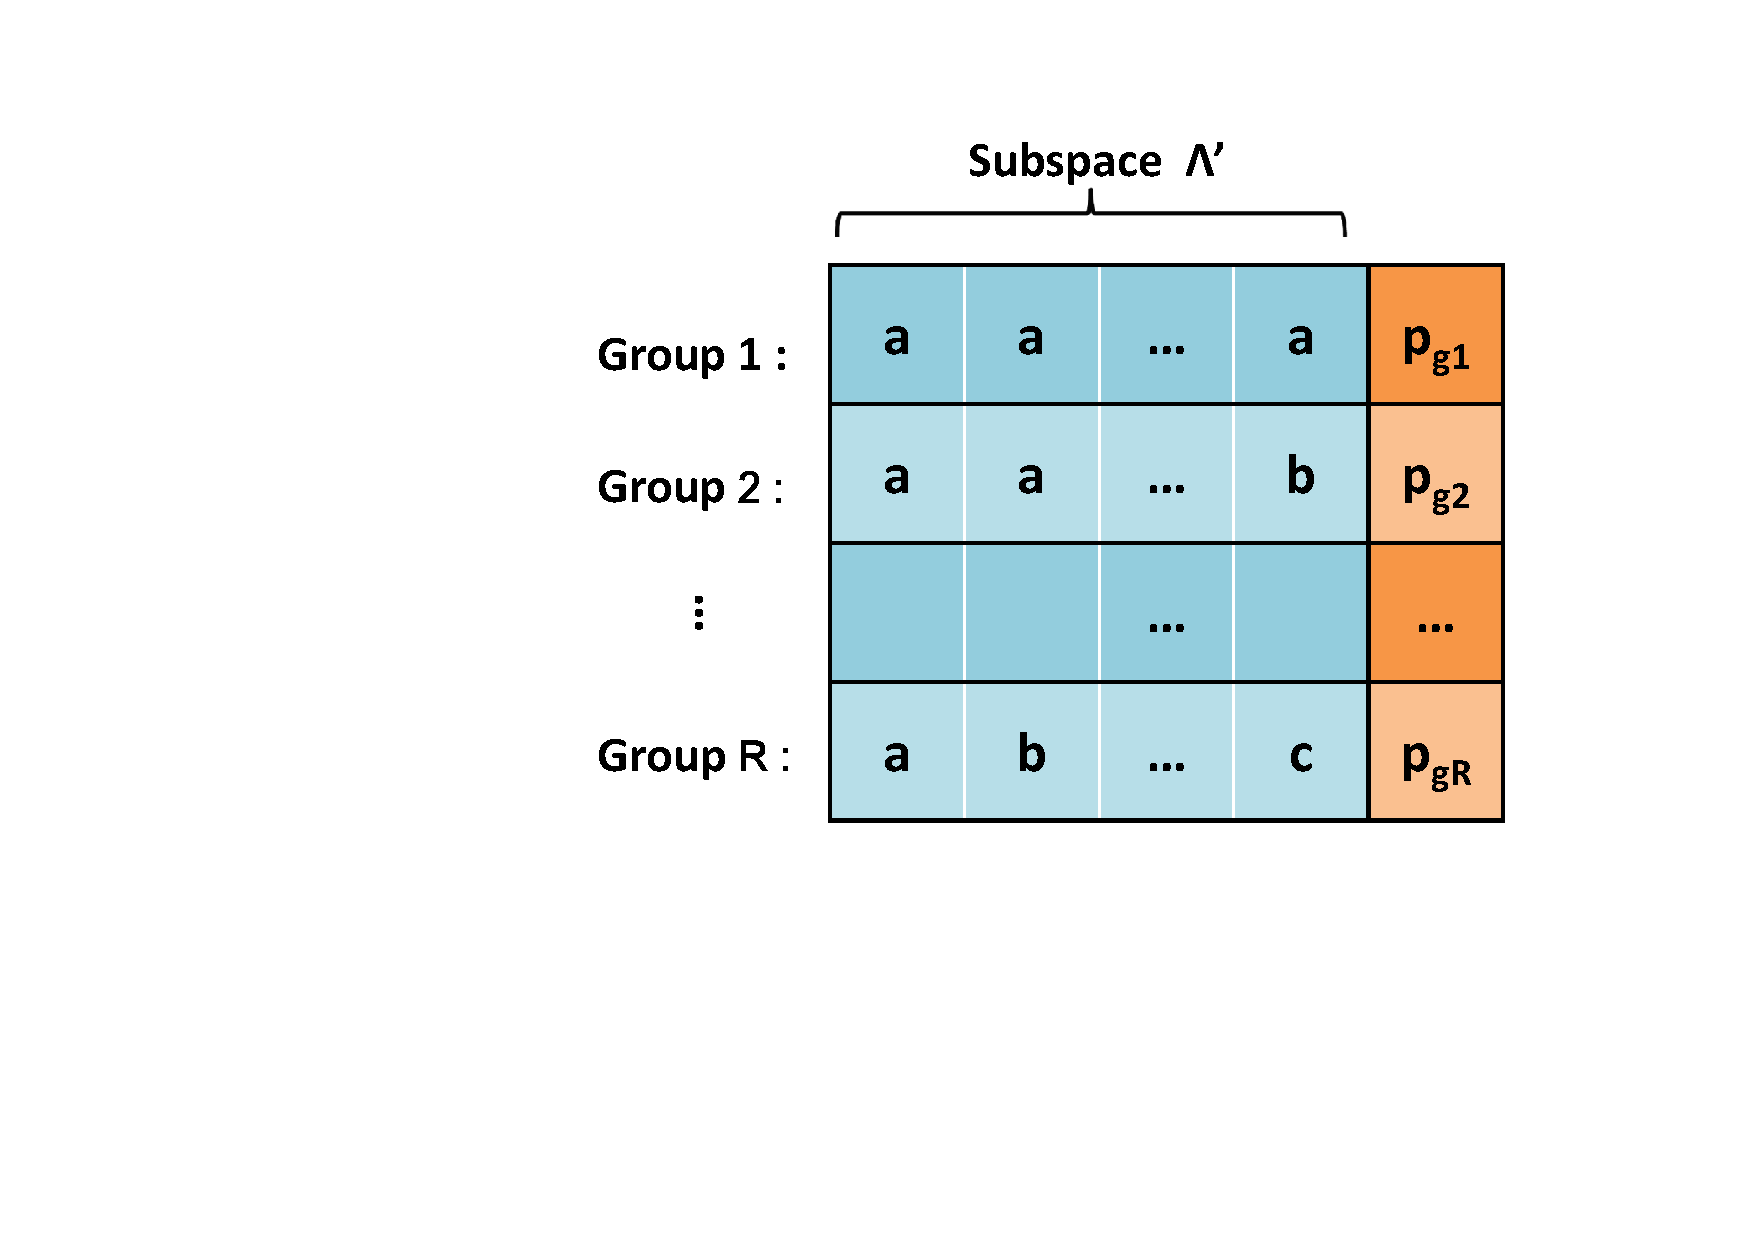
\includegraphics[width = 0.6\columnwidth]{figure/codebook.pdf}
\vspace{-3mm}
\caption{The codebook of an attribute matrix}
\label{fig:codebook}
\end{figure}

\noindent \textbf{Coding cost of the non-cluster area $CC(U)$:} The Non-cluster area consists of the elements in the adjacency matrix $A$ and the attributed matrix $F$ that are not contained in $K$ clusters, which are represented as $U_A$ and $U_F$ respectively. Similarly, the coding cost of the non-cluster area $CC(U)$ is the sum of the structural coding cost $CC(U_A)$ and the attributed coding cost $CC(U_F)$, as shown in Eq.(\ref{eq:nc}). 
\begin{equation}
CC(NC) = CC(U_A) + CC(U_F)
\label{eq:nc}
\end{equation}

We consider all elements of the structural non-cluster area $U_A$ entirely and code them with a fixed coding order. The coding cost of the non-cluster area of the structural aspect $CC(U_A)$ can be encoded as shown Eq.\ref{eq:unclusterA}. Here, $p_1(U_A)$ is the number of edges in $U_A$ and $p_0(U_A)$ is the number of no-egdes in $U_A$. Due to the symmetry property of the matrix, $n_{U_A} = \frac{N_{U_A}\cdot(N_{U_A}-1)}{2}$ is equals to half of the elements in the non-cluster area. 
\begin{equation}
CC(U_A)= -n_{U_A}\cdot (p_1(U_A)\cdot \log_2 p_1(U_A) + p_0(U_A) \cdot \log_2 p_0(U_A)).
\label{eq:unclusterA}
\end{equation}

In the non-cluster area of attribute aspect $U_F$, we encode the remaining categories of each attribute one by one. The coding cost $CC(U_F)$ is calculated in Eq.\ref{eq:unclusterF}, where $N_{\lambda_i}$ is the number of categories of attribute $\lambda_i$ that are not assigned to any clusters, and $p_{\theta_j}$ is the probability of an category $\theta_j$ in the remaining elements of the corresponding attribute. 
\begin{equation}
CC(U_F)= -\sum^T_{i=1}\sum^{\theta_j}_{j=1} N_{\lambda_i}\cdot p_{\theta_j}\cdot \log_2 p_{\theta_j} .
\label{eq:unclusterF}
\end{equation}

\subsubsection{Model Cost $L(M)$}
\noindent For encoding the model cost $L(M)$ of the attributed graph, every cluster will be compressed in three aspects: the assignments of each vertex , the  assignments of each attribute and the parameters of the clusters.
\\

\noindent \textbf{Coding cost of vertices assignment $CC_{IDV}(C_i)$: } As overlapping is allowed in our proposed algorithm, a vertex can be assigned to multiple clusters. For each cluster, we adopt an assignment list to label the existence of vertices. An example for this is shown in Figure \ref{fig:list}. When the vertex belongs to the cluster, the corresponding value in the list is set to $``1"$, otherwise set to $``0"$. Therefore, the coding cost of the vertices assignment for a cluster $CC_{IDV}(C_i)$ is lower bounded by its entropy as shown in Eq.(\ref{eq:nodeid}), where $p_{1}(L)$ and $p_{0}(L)$ denote the probability of $1$ and $0$ in the assignment list of cluster $C_i$ respectively, and $N$ is the number of vertices in the graph. Then the coding cost of the vertice assignments of the whole graph is the sum of cost for all clusters.
\begin{equation}
CC_{IDV}(C_i)= - N \cdot ( p_{1}(L) \cdot \log_2 {p_{1}(L)} +  p_{0}(L) \cdot \log_2 {p_{0}(L)}).
\label{eq:nodeid}
\end{equation}

\begin{figure}[h]
\centering
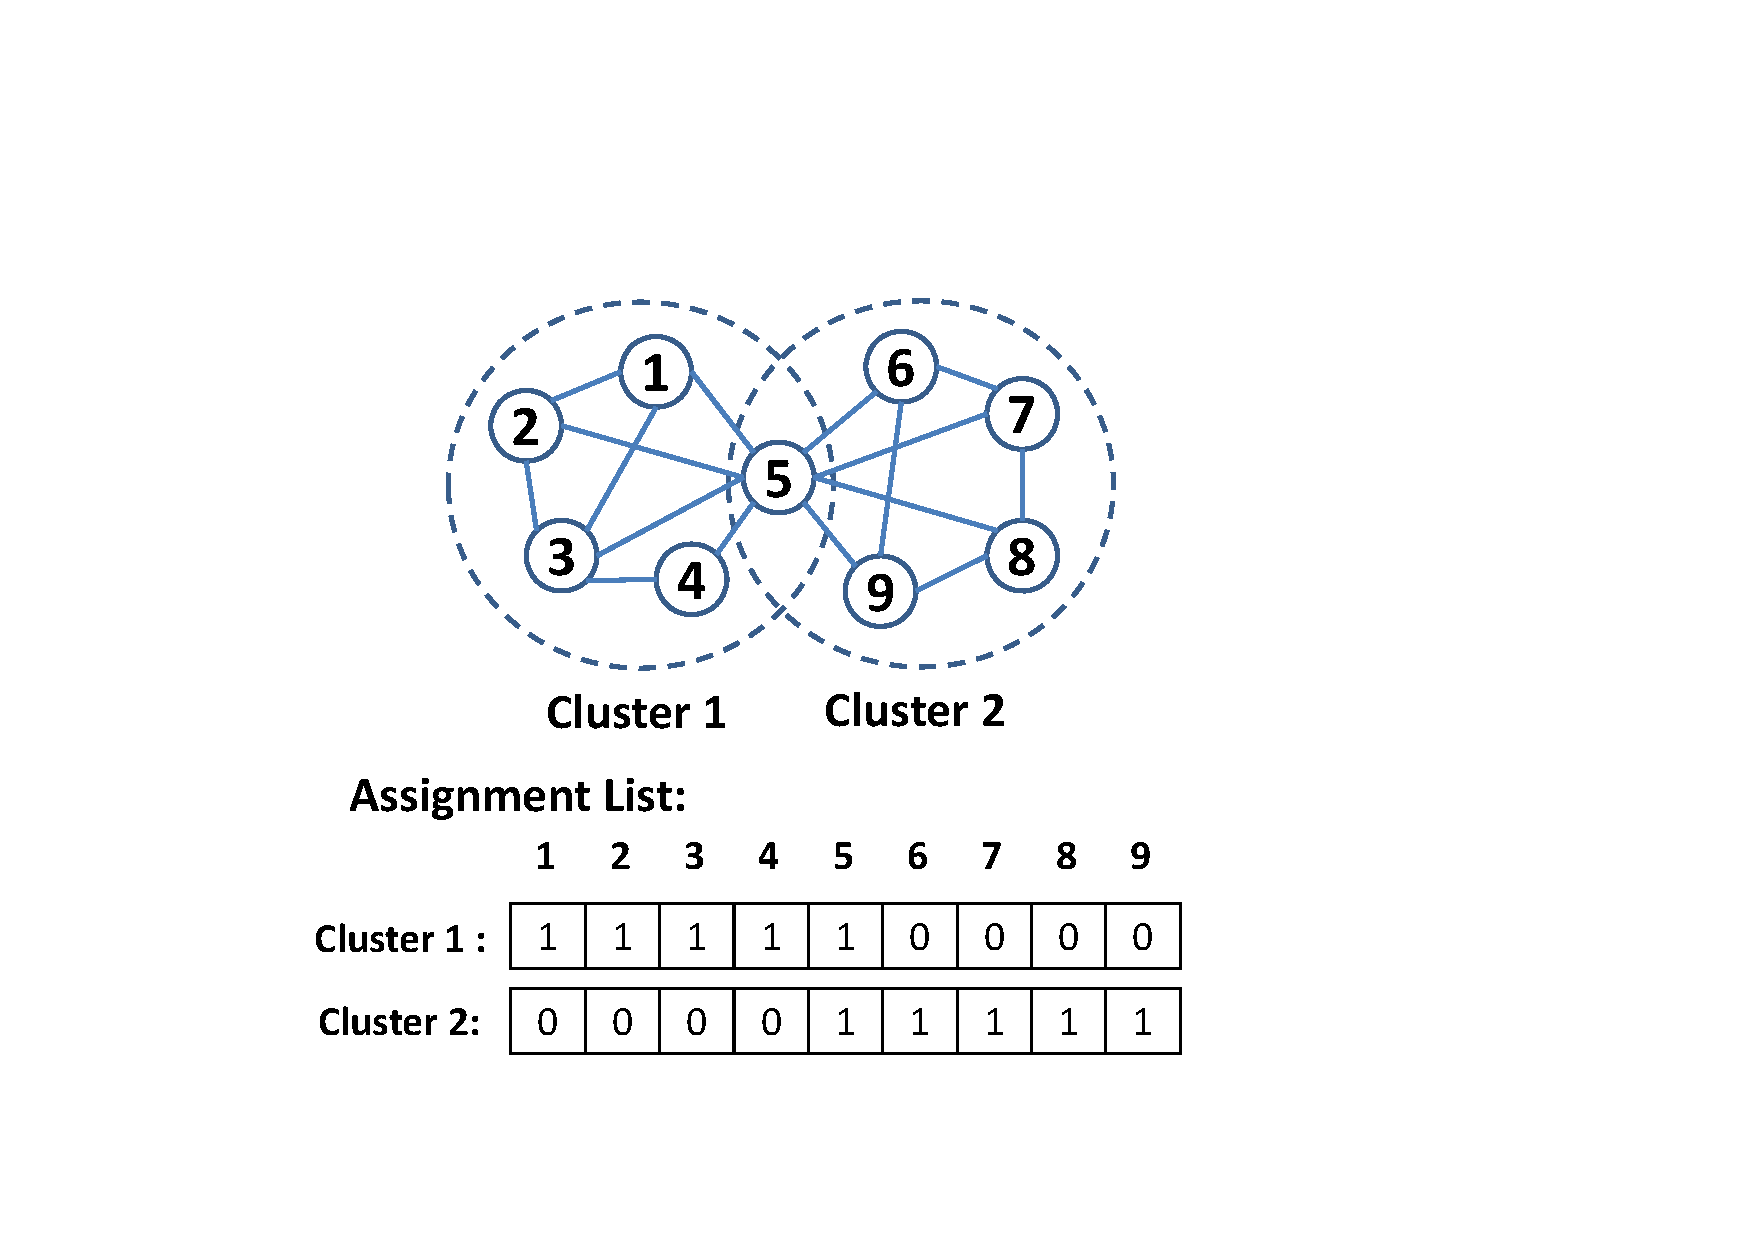
\includegraphics[width = 0.7\columnwidth]{figure/list.pdf}
\vspace{-3mm}
\caption{The assignment list of vertices}
\label{fig:list}
\end{figure}

\noindent \textbf{Coding cost of attributes assignments $CC_{IDF}(C_i)$: }
In our proposed algorithm, the corresponding attribute subspaces of clusters are also detected. Similarly, there is overlapping among the subspaces as well, which means an attribute can be grouped into multiple clusters. Here we also adopt an assignment list with size $T$ to represent attributes that are contained in a subspace of a cluster, which is shown in Eq.(\ref{eq:featureid}).
\begin{equation}
CC_{IDF}(C_i)= - T \cdot ( p_{1}(L) \cdot \log_2 {p_{1}(L)} + p_{0}(L) \cdot \log_2 {p_{0}(L)}).
\label{eq:featureid}
\end{equation}

\noindent \textbf{Coding cost of parameters:} To ensure that the receiver acquires the complete information, all parameters need to be encoded to keep the lossless compression. The cost of these parameters can be calculated from Eq.(\ref{eq:nodepara}), where $n_p$ is the number of parameter and $n_E$ is the number of entries. 
\begin{equation}
CC_{para}= 0.5 \cdot n_p \cdot \log_2 n_E.
\label{eq:nodepara}
\end{equation}

First, we need to encode the probability of $``1"$s and $``0"$s in each cluster $C_i$ and of the non-cluster area $U$. Here $n_p = K + 1$ and $n_E$ is equals to half of the entries of the corresponding subset adjacency matrix $A_{C_i}$. Secondly, we encode he probabilities of  the $R$ groups in the codebook. Here $n_p = R-1$ and $n_E$ are equals to the number of categories of the codebook. Thirdly, in the non-cluster area of the attribute matrix, we encode the probabilities of all categories in each attribute as parameter, for each attribute $i$. For this $n_p = \theta_j -1$ and $n_E$ are equals to the size of the remaining categories of attribute $i$. Finally, we encode the probabilities of the assignment lists as parameters as well, here $n_p = 1$ and $n_E$ are equals to the size of the list. 

%\subsubsection{Cost of Adjacency Matrix $A$}



%The adjacency matrix $A$ embodies structural information with $1$ and $0$ denoting the existence of edges. Suppose $K$ clusters $C=\{C_1,C_2,...,C_K \}$ are discovered from an attributed graph $G$. Then for every cluster in $C$ we need to encode all vertices that are included in that cluster, more specifically we encode the cluster ID the vertices belong to in $CC^A_{ID}$. For doing so we adopt an assignment list with size $N$ to label the existence of vertices in every cluster. When the vertex belongs to a cluster , the corresponding value in the list is set to $1$, or set to $0$. Therefore, the coding cost for the cluster ID of vertices in a cluster $C_i$ is lower bounded by its entropy as shown in Eq.\ref{eq:nodeid}  where $P_{ID}(1)$ in the assignment list of $C_i$ denotes the probability of $1$ while $P_{ID}(0)$ denotes the probability of $0$.
%\begin{equation}
%CC^A_{ID}(C_i)= N \cdot (P_{ID}(1) \cdot log_2 \frac{1}{P_{ID}(1)} + P_{ID}(0) \cdot log_2 \frac{1}{P_{ID}(0)}).
%\label{eq:nodeid}
%\end{equation}
%
%Eq.\ref{eq:clusterA} shows the coding cost of the structural information of each cluster $C_i$, where $P(1)$ and $P(0)$ stands for the probability if a $1$ and respectively a $0$ is standing in the adjacency matrix of cluster $C_i$. $n_{C_i}=\frac{N_{C_i}(N_{C_i}-1)}{2}$ is the number of entries in cluster $C_i$.
%
%\begin{equation}
%CC^A(C_i)= n_{C_i}\cdot (P(1)\cdot log_2 \frac{1}{P(1)} + P(0)\cdot log_2 \frac{1}{P(0)}).
%\label{eq:clusterA}
%\end{equation}
%
%To ensure that the receiver of the compression is acquiring the complete information, all probabilities of the occurrence of $1$ and $0$ in each cluster $C_i$ need to be encoded as two parameters. The cost of these parameters can be calculated from Eq.\ref{eq:nodepara}, where $n_p$ is number of parameter of Cluster $C_i$ and $n_E$ is the number of entries. In cluster $C_i$, $n_E=\frac{N_{C_i}(N_{C_i}-1)}{2}$ is the number of entries, $n_p =2$.
%\begin{equation}
%CC^A_p(C_i)= \frac{n_p-1}{2} \cdot log_2 n_E.
%\label{eq:nodepara}
%\end{equation}
%
%After $K$ clusters are generated by IROC, no-cluster area is consist of all elements in the adjacency matrix $A$ which are not contained in $K$ clusters.. We consider it as an ensemble and calculate its edge probability to receive a loseless compression. Therefore, we need to encode the no-cluster area $U_A$ as in Eq.\ref{eq:unclusterA}, where $P_{U_A}(1)$ is the number of links in $U_A$ and $P_{U_A}(0)$ is the number of disconnection in $U_A$, $n_{U_A} = \frac{N_{U^A}(N_{U^A}-1)}{2}$ is the number of elements in the no-cluster area. Similarly, the parameter costs $CC_p(U_A)$ of $P_{U_A}(1)$ and $P_{U_A}(0)$ can be calculated from Eq.\ref{eq:nodepara}. Again, $n_E = n_{U_A}$ is number of entries in $U_A$ and $n_p = 2$.
%\begin{equation}
%CC(U_A)=n_{U_A}\cdot (P_{U_A}(1)\cdot log_2 \frac{1}{P_{U_A}(1)} + P_{U_A}(0) \cdot log_2 \frac{1}{P_{U_A}(0)}).
%\label{eq:unclusterA}
%\end{equation}
%By all accounts, the coding cost of the adjacency matrix $A$ is exhibited in Eq.\ref{eq:adjcc}.
%
%\begin{equation}
%\begin{split}
%CC^A = \sum_{i=1}^K (CC^A_{ID}(C_i) + CC^A_p(C_i) + CC^A(C_i)) \\+ CC(U_A) + CC_p(U_A).
%\end{split}
%\label{eq:adjcc}
%\end{equation}
%
%
%%\subsubsection{Cost of an Attribute Matrix $F$}
%From the attribute matrix $F$ we are not only obtaining information about the node clusters, but also about the subspace of attributes of each cluster. Because the information of node clusters has already been encoded in the adjacency matrix, only the information of the attributes needs to be encoded in the attributed matrix. Figure \ref{fig:codebook} describes a codebook of an attributed matrix with the cluster $C_i$. $\Lambda'$ being the attribute subspace in which the subset of attributes is $\Lambda$. Every vertex possesses a category in each attribute of the subspace. Equally, in cluster $C_i$, the attributes of a vertex are a category string with a size equal to the subspace. Suppose attribute of $N_{C_i}$ vertex can be formed into $R$ groups and the percentages of each group in a cluster can be calculated as $P_{F1},P_{F2},...,P_{FR}$. Then the information of the attributes of cluster $C_i$ can be encoded as Eq.\ref{eq:clusterF}.
%\begin{figure}[h]
%\centering
%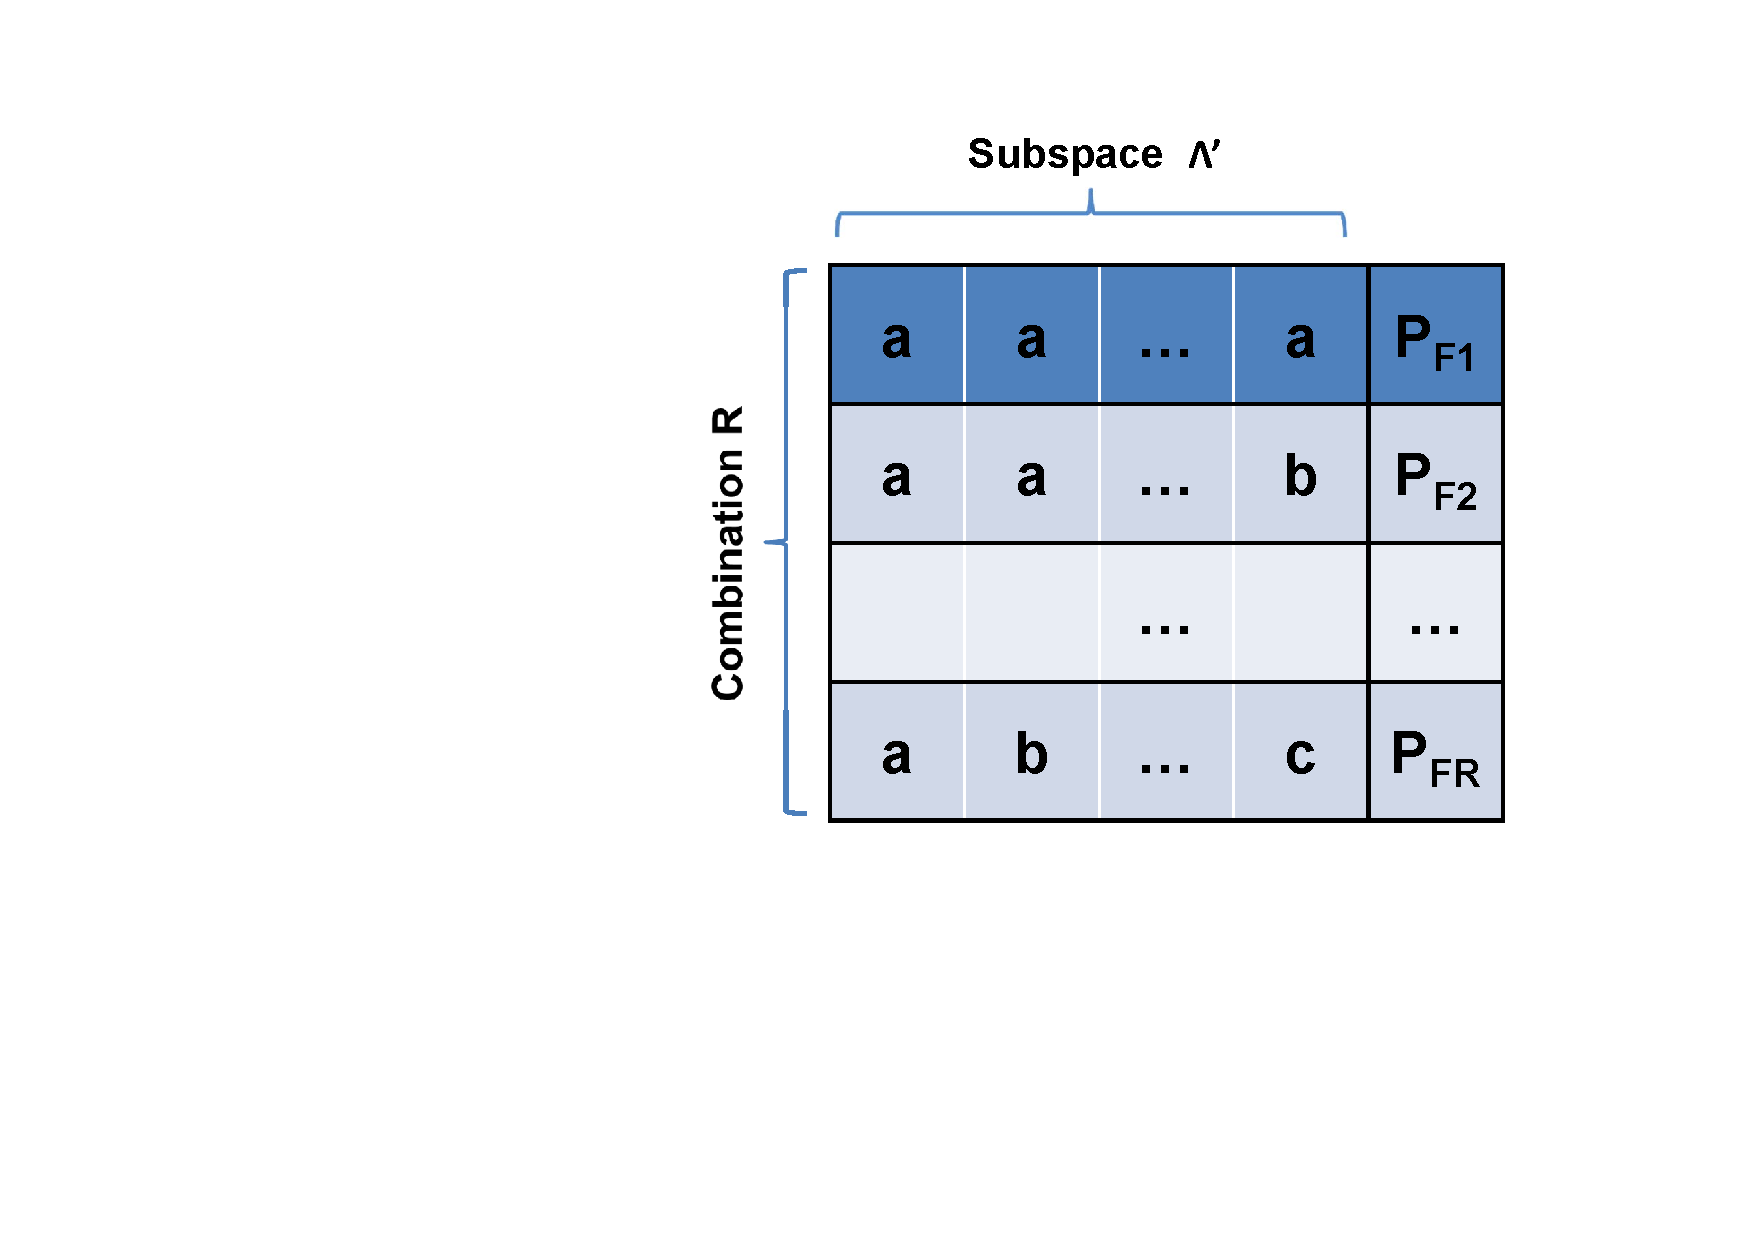
\includegraphics[width = 0.5\columnwidth]{figure/codebooka.pdf}
%\vspace{-3mm}
%\caption{The code book of an attribute matrix}
%\label{fig:codebook}
%\end{figure}
%
%\begin{equation}
%CC^F(C_i)= R \cdot \sum_{i=1}^R P_{Fi}\cdot log_2 \frac{1}{P_{Fi}}
%\label{eq:clusterF}
%\end{equation}
%
%Moreover, the probabilities of a group are encoded as parameter with the cost being calculated from Eq.\ref{eq:nodepara}, where the number of parameters $n_p$ is $R$, and $n_E$ is the number of vertex in cluster $C_i$. Additionally, we use $log_2 \theta_k$ bits to encode a category in a attribute $\lambda_k$. The parameter costs $CC^F_p(C_i)$ of an attribute matrix of a cluster $C_i$ is calculated as is shown in Eq.\ref{eq:Fpara}.
%
%\begin{equation}
%CC^F_p(C_i)= \frac{R -1}{2} \cdot  log_2 N_{C_i} + N_{C_i} \cdot \sum_{i=1}^S log_2 \theta_k.
%\label{eq:Fpara}
%\end{equation}
%
%Similarly, there is also overlapping among the subspaces of clusters. Therefore, we adopt a list with size $ T $ to represent attributes which are contained in a subspace of a cluster.  If the subspace of a cluster includes the attribute, the corresponding value of the list is set as $1$, or set as $0$. Also, the coding cost of the subspace ID of a cluster  $CC^F_{ID}(C_i)$ is calculated from Eq.\ref{eq:featureid}, where $P_S(1)$ denotes in the list of $C_i$ the probability of $1$ which means the attribute is contained in the subspace , and $P_S(0)$ denotes the probability that this attribute is not contained in the subspace -therefore its value is $0$.
%
%\begin{equation}
%CC^F_{ID}(C_i)= T \cdot (P_S(1) \cdot log_2 \frac{1}{P_S(1)} + P_S(0) \cdot log_2 \frac{1}{P_S(0)}).
%\label{eq:featureid}
%\end{equation}
%%
%%and,
%%
%%\begin{equation}
%%\small
%% CC^F' =
%%\label{eq:featureid}
%%\end{equation}
%
%In addition, the no-cluster areas of the attribute matrix are categories of each attribute which are not contained in the clusters. Therefore, we again encode the remaining categories of each cluster for loseless compression as shown in Eq.\ref{eq:unclusterF}, where $N_{\lambda_i}$ is the number of categories of attribute $\lambda_i$ which are not assigned to clusters, and $P_{U_F}(\theta_j)$ is the probability of each category occupied in the remaining elements. Each attribute contains the remaining probabilities of a category, and these probabilities are encoded as parameters which can be calculated from Eq.\ref{eq:unodepara}.
%\begin{equation}
%CC(U_F)= \sum^T_{i=1}\sum^{\theta_j}_{j=1} N_{\lambda_i}\cdot P_{U_F}(\theta_j) \cdot log_2 \frac{1}{P_{U_F}(\theta_j)} .
%\label{eq:unclusterF}
%\end{equation}
%
%\begin{equation}
%CC^F_p(U_F)= \sum^T_{i=1} \frac{\theta_i -1}{2} \cdot log_2 N_{\lambda_i}.
%\label{eq:unodepara}
%\end{equation}
%
%Consequently, the cost of an attribute matrix $F$ is shown in Eq.\ref{eq:attributecc}. Overall the coding cost of an attributed graph $G$ is the sum of costs of the adjacency matrix and the attributed matrix as can be seen in Eq.\ref{eq:cc}.
%\begin{equation}
%\begin{split}
%CC^F = \sum_{i=1}^K (CC^F_{ID}(C_i) + CC^F_p(C_i) + CC^F(C_i))\\
% + CC(U_F) + CC_p(U_F).
%\end{split}
%\label{eq:attributecc}
%\end{equation}
%With that the overall cost can be calculated:
%\begin{equation}
%CC = CC^A + CC^F.
%\label{eq:cc}
%\end{equation}





\section{Algorithm IROC}
%The pivotal procedural of detecting overlapping community is how to assign vertex to multiple community. In this paper, we achieve vertex overlapping by constructing redundancy from small subgraphs.
\noindent In this section, we propose an effective and efficient searching algorithm IROC to detect overlapping clusters in an attributed graph. The initialization phase and the refinement phase are the two key steps in IROC. The initialization phase is again divided into two subroutines for a) creating graph substructures and b) finding their coherent attribute subspace. The refinement phase takes the responsibility of improving the quality of initial clusters by a) removing redundant parts of the cluster and b) reassigning vertices between two clusters. 

\subsection{Initialization}
\noindent \textbf{Creating Graph Substructures}: The idea for the implicit creation of an overlapping graph structure is to create small redundant subgraphs. Each small subgraphs is simply composed of a vertex and all its neighbors. This is an intuitive way to obtain all these small redundant subgraphs. Therefore, $N$ subgraphs with overlapping vertices are extracted from an attributed graph $G$, where $N$ is the number of vertices in $G$. First of all, in order to eliminate over much redundancies we select $K_s$ subgraphs as initial rough clusters based on the MDL principle automatically. The procedure is shown in Algorithm \ref{alg:Initialization}. To be specific, we consider $N$ subgraphs as rough clusters. And we consider there is no clusters in the attributed graph $G$. Then we add a rough cluster to the clusters $C$ and calculate the coding cost by Eq.(\ref{eq:mdl}) one by one. After that we select the cluster with the minimum coding cost as the first cluster. We keep the selected cluster in the clusters $C$. Analogously, in the remaining $N-1$ candidates, we try to add each candidate as the second cluster and choose the one with the minimum coding cost repetitively. This process stops until all vertices are processed, so that $K_s$ initial clusters are chosen automatically.
\\

\noindent \textbf{Finding a Coherent Attribute Subspace}: After obtaining $K_s$ rough clusters, we also need to find out the attribute subspace of each rough clusters. Algorithm \ref{alg:findsubspace} demonstrates the progress of searching an attribute subspace of a cluster $C_i$ based on the MDL principle. Every vertex of a rough cluster possesses a category in each attribute. For each cluster, we calculate the entropy of each attribute to measure the purity of the categories in the attribute. Entropy in this case refers to the consistence of categories of an attribute. The lower the value, the higher the consistency of the attribute. Thus we order the attributes in ascending order of their entropies. If some attributes possesses the same value, they are formed into groups and considered as one candidate. Thus the candidates of attributes are form as $\Lambda^o=\{\Lambda^o_1,\Lambda^o_2,...,\Lambda^o_{T_g} \}$. Based on the prerequisite that the subspace of the cluster is initialized with an empty set, we add the ordered attribute candidates to the subspace one by one, and meanwhile calculate the coding cost of the whole graph $G$ by Eq.(\ref{eq:mdl}). Then we select the attribute subspace $\Lambda'$ of a cluster $C_i$ with the minimum coding cost. The attribute subspace of the cluster is fixed after chosen. In the same way, the attribute subspace of other $K_s-1$ clusters are chosen.   

\begin{algorithm}[htbp]
\caption{\textbf{Creating Subgraphs}}
\label{alg:Initialization}
\begin{algorithmic}[1]
\REQUIRE
    Attributed Graph $G$ with $N$ Vertices and $T$ Attributes 
\ENSURE
    $K_s$ Rough Clusters: $C =\{C_1,C_2,...,C_{K_s}\}$
\STATE Construct $N$ subgraphs $SS = \{ss_1,ss_2,...,ss_N \}$ as initial $N$ clusters;
\STATE $C \leftarrow \emptyset$;
\WHILE{All vertices are ergodic}
\FOR{All substructures in $SS$}
\STATE Calculate coding cost of $ss_i \bigcup C$;
\ENDFOR
\STATE Select $ss_m$ with minimum coding cost, $ss_m \bigcup C$;
\STATE Remove $ss_m$ from $SS$;
\ENDWHILE
\RETURN {$K_s$ Rough Clusters: $C =\{C_1,C_2,...,C_{K_s}\}$}.
\end{algorithmic}
\end{algorithm}

\begin{algorithm}[htbp]
\caption{\textbf{Finding Subspace}}
\label{alg:findsubspace}
\begin{algorithmic}[1]
\REQUIRE
    A Cluster $C_i$ with $N_c$ Vertices and $T$ Attributes
\ENSURE
    Subspace $\Lambda' = \{\lambda'_1,\lambda'_2,...,\lambda'_S \}$

\STATE $\Lambda'\leftarrow\emptyset$;
\FOR{$i$ from $1$ to $T$}
\STATE Calculate entropy of each attribute $\lambda_i$;
\ENDFOR
\STATE Group attributes with same entropy and arrange attributes in ascending order $\Lambda^o=\{\Lambda^o_1,\Lambda^o_2,...,\Lambda^o_{T_g} \}$;
\FOR{$i$ form $1$ to $T_g$}
\STATE $\Lambda^o_i\bigcup \Lambda'$, and calculate coding cost of all clusters $CC$.
\IF {$CC$ increases}
\STATE break;
\ENDIF
\ENDFOR
\RETURN {Subspace $\Lambda' = \{\lambda'_1,\lambda'_2,...,\lambda'_S \}$}.
\end{algorithmic}
\end{algorithm}

\subsection{Refinement}
\noindent \textbf{Removing Redundancy:} After the initialization step, we receive $K_s$ small attributed clusters which contain \emph{redundant} information. These redundancies serve to generate and find the overlapping in the beginning but are later unwelcome. Therefore our heuristic bottom up algorithm needs to merge these small initial rough clusters to remove redundancies. We define an information-theoretic based similarity which measures the degree of the redundancy between every pair of clusters. Due to the fact that both structural and attribute information are present, we measure the similarity of two clusters as shown in Eq. (\ref{eq:similarity}):
\begin{equation}
Sim(C_i,C_j) = H(O_A)+ H(O_F).
\label{eq:similarity}
\end{equation}
where $H(\cdot)$ is entropy defined in Eq. (\ref{eq:entropy}), $O_A$ and $O_F$ are the structural and attribute overlapping part of cluster $C_i$ and $C_j$ respectively. This quality function tackles the chief problem of merging two cluster: the amount of overlaps in structural and attribute information. How can two cluster be merged without creating new redundancy if they are overlapping in structure and attribute space? On the structural aspect, entropy paysoff the denser the overlapping area. Also the smaller the entropy, the denser the overlapping part of the cluster. Thus the smaller entropy of structural overlapping part leads us to detect dense clusters. While on the attribute side, the entropy measures the purity of categories in the overlapping area of the attributes. This ensures that the cluster is provided with same categories in the attributes. The smaller the entropy is, the higher the similarity of the attributes in the overlapping part is. Thus the smaller entropy of  attribute overlapping part leads us to detect clusters with coherent meaning. Therefore, the defined similarity balances the entropy of the two aspects, which guides us to merge the two most similar clusters. And in every search run we merge the pair of clusters that have a minimal similarity.
\\

\noindent \textbf{Assigning Vertices:} Obviously, merging two clusters $C_i$ and $C_j$ to form a new cluster $C_{new}$ is able to remove redundancy. However, such merging may not eliminate all redundancies. Depending on how accurate the removing of the redundancy works, we need to modify the cluster further in a second refinement step which is shown in Algorithm \ref{alg:av}. For all vertices $\{v_1,v_2,...,v_{N_{C_{new}}}\}$ in $C_{new}$, we try to split a vertex $v_1$ from $C_{new}$ and consider it as a new cluster $C_{split}=\{v_1\}$. Then we find the subspace of $C_{split}$ and refine the subspace of $C_{new}=\{v_2,...,v_{N_{C_{new}}}\}$. If such process reduce the coding cost, we keep the modification and try to move the next vertex $v_2$ from $C_{new}$ to $C_{split}$. If the coding cost is not reduced, we move the vertex $v_1$ back to $C_{new}$. The refinement of cluster $C_{new}$ ends when the coding cost achieves its local minimum. If cluster $C_{split}$ is not empty, we treat $C_{split}$ as a new candidate and add it to the clusters. 

\begin{algorithm}[htbp]
\caption{\textbf{Assigning Vertices}}
\label{alg:av}
\begin{algorithmic}[1]
\REQUIRE
    Cluster $C_{new}$
\ENSURE
    Cluster $C_{new}$ and Cluster $C_{split}$
\STATE Creat a cluster $C_{split}$, $C_{split} \leftarrow \emptyset$;
\STATE Calculate coding cost of all the clusters $CC$;
\FOR{All nodes in $C_{new}$}
\STATE $v \in C_{new}$, remove $v$ from $C_{new}$, add $v$ to $C_{split}$;
\STATE \textbf{Finding Subspace} of $C_{split}$ and $C_{new}$;
\STATE Calculate coding cost of all the clusters $CC_{new}$
\IF{$CC_{new}$ $>$ $CC$}
\STATE Restore $v$ to $C_{new}$;
\ENDIF
\ENDFOR
\RETURN {$C_{new}$ and $C_{split}$}.
\end{algorithmic}
\end{algorithm}
 
\subsection{IROC}
\noindent The overall procedure of IROC is shown in Algorithm \ref{alg:GraphClustering}. First, we automatically select $K_s$ rough clusters and search their attribute subspace as described in the initialization phase. Then we calculate the similarity of every pair of clusters, and merge the two cluster with a minimum similarity. After that a new cluster $C_{new}$ is formed and we find the subspace of it. Then we try to assign vertices from $C_{new}$ to $C_{split}$ under the control of MDL. And we consider $C_{split}$ as a new cluster and recalculate the similarity of every pair of clusters. The merging process continues iteratively and is ended when the coding cost of all clusters achieve its local minimum. Finally, $K$ clusters with coherent attribute subspaces without redundancy are output.

\begin{algorithm}[htbp]
\caption{\textbf{IROC}}
\label{alg:GraphClustering}
\begin{algorithmic}[1]
\REQUIRE
    Attributed Graph $G$
\ENSURE
    $K$ Clusters with Subspace $C = {C_1, C_2,...,C_K}$
\STATE \textbf{Creating Subgraphs} $C = {C_1, C_2,...,C_{K_s}}$ ;
\FOR{$i$ from 1 to $K_s$}
\STATE \textbf{Finding Subspace} of $C_i$
\ENDFOR
\WHILE {Converge}
\STATE Calculate similarity of every pair of clusters;
\STATE Merge two most similar clusters as $C_{new}$;
\STATE \textbf{Finding Subspace} of $C_{new}$;
\STATE \textbf{Assigning Vertices} of $C_{new}$;
\ENDWHILE
\RETURN {$C = {C_1, C_2,...,C_K}$}.
\end{algorithmic}
\end{algorithm}

\subsection{Complexity Analysis}
\noindent Suppose we have an attributed graph $G$ with $N$ vertices, $E$ edges and $T$ attributes for each vertex. We first analyse the complexity of the coding when we have $K$ clusters. For each clusters we need to count the edges of the cluster and go through its vertices and attributes to get the probability distributions. The complexity of these processes for all clusters are $O((K+1)\cdot(A_v{_E}+A_v{_N}\cdot A_v{_T}))$, where $A_v{_E} < E$ is the average number of edges, $A_v{_N} < N$ is the average number of vertices and $A_v{_T} < T$ is the average number of subspace attributes. The multiplier factor is $K+1$ considering the no-cluster area. Since the number of cluster is $K \ll N$, the complexity of the proposed coding scheme is $O(E+N\cdot T)$.

In initialization phase of IROC, we greedily choose the initial clusters, since their attributes are not considered in this part, the complexities are $O(K_s\cdot N)$ and $O(N\cdot E)$ respectively, where $K_s$ is the number of initial clusters. Then we need to find the subspace for each cluster. In this part only attributes are considered, its complexity is $O(K_s \cdot N\cdot T^2)$. The reason is that for each cluster we need to calculate the coding cost $T$ times. Finally, the complexity of the full initialization phase (both parts combined) is $O(K_s(N + N\cdot T^2))$ for the random one and $O(K_s\cdot N(E+T^2))$ for the greedy approach.

In the full refinement step, we need to process $K_s^2$ pairs of clusters. In each merging and splitting process, we need to move vertices to other clusters and then calculate the subspace of the new clusters. Therefore, we need $O(N^2\cdot T^2)$ time to do so. Finally, the complexity in this step is $K_s^2\cdot O(N^2\cdot T^2)$.




\section{Experiments}
In this section, we evaluate our proposed algorithm IROC on both synthetic data sets and real data sets and compare it with $4$ relevant algorithms. The code of the comparison methods are obtained from the authors. Experiments have been performed on a workstation with $2.9GHz$ Intel Core $i7$ and $8G$ memory.

\subsection{Synthetic Data sets}
\subsubsection{Data sets}
The sketches of three synthetic data sets are shown in Tab. \ref{tab:syn}. Each circle represents a densely connected cluster and the shadow part denotes the overlapping part in which vertices are assigned to multiple clusters. The synthetic attributed graphs are generated with the following parameters: Each cluster contains $200$ vertices ($n_c = 200$); $n_o$ is the number of vertices in the overlapping part; the density of edges in and between clusters are $0.8$ and $0.1$ respectively ($d_c=0.8, d_b=0.1$). The subspace of attributes of the three synthetic data sets are also shown in Table \ref{tab:syn}. The number of dimensionality of the subspace of each cluster is denoted as $n_d$ and $2$ dimensions are overlapping ($n_{od} = 2$). Each cluster contains nearly same category in its subspace attributes and $r=0.05$ of them are randomly generated with other categories. The categories which do not belong to the subspace are randomly generated. 
\begin{table*}[t]
\centering
\caption{Parameter Settings for Generating Synthetic Data Set}
\begin{tabular}{|c|c|c|c|}
\hline
Datasets & Syn1 & Syn2 & Syn3\\
\hline
\tabincell{c}{Sketch} & \raisebox{-0.9\height}{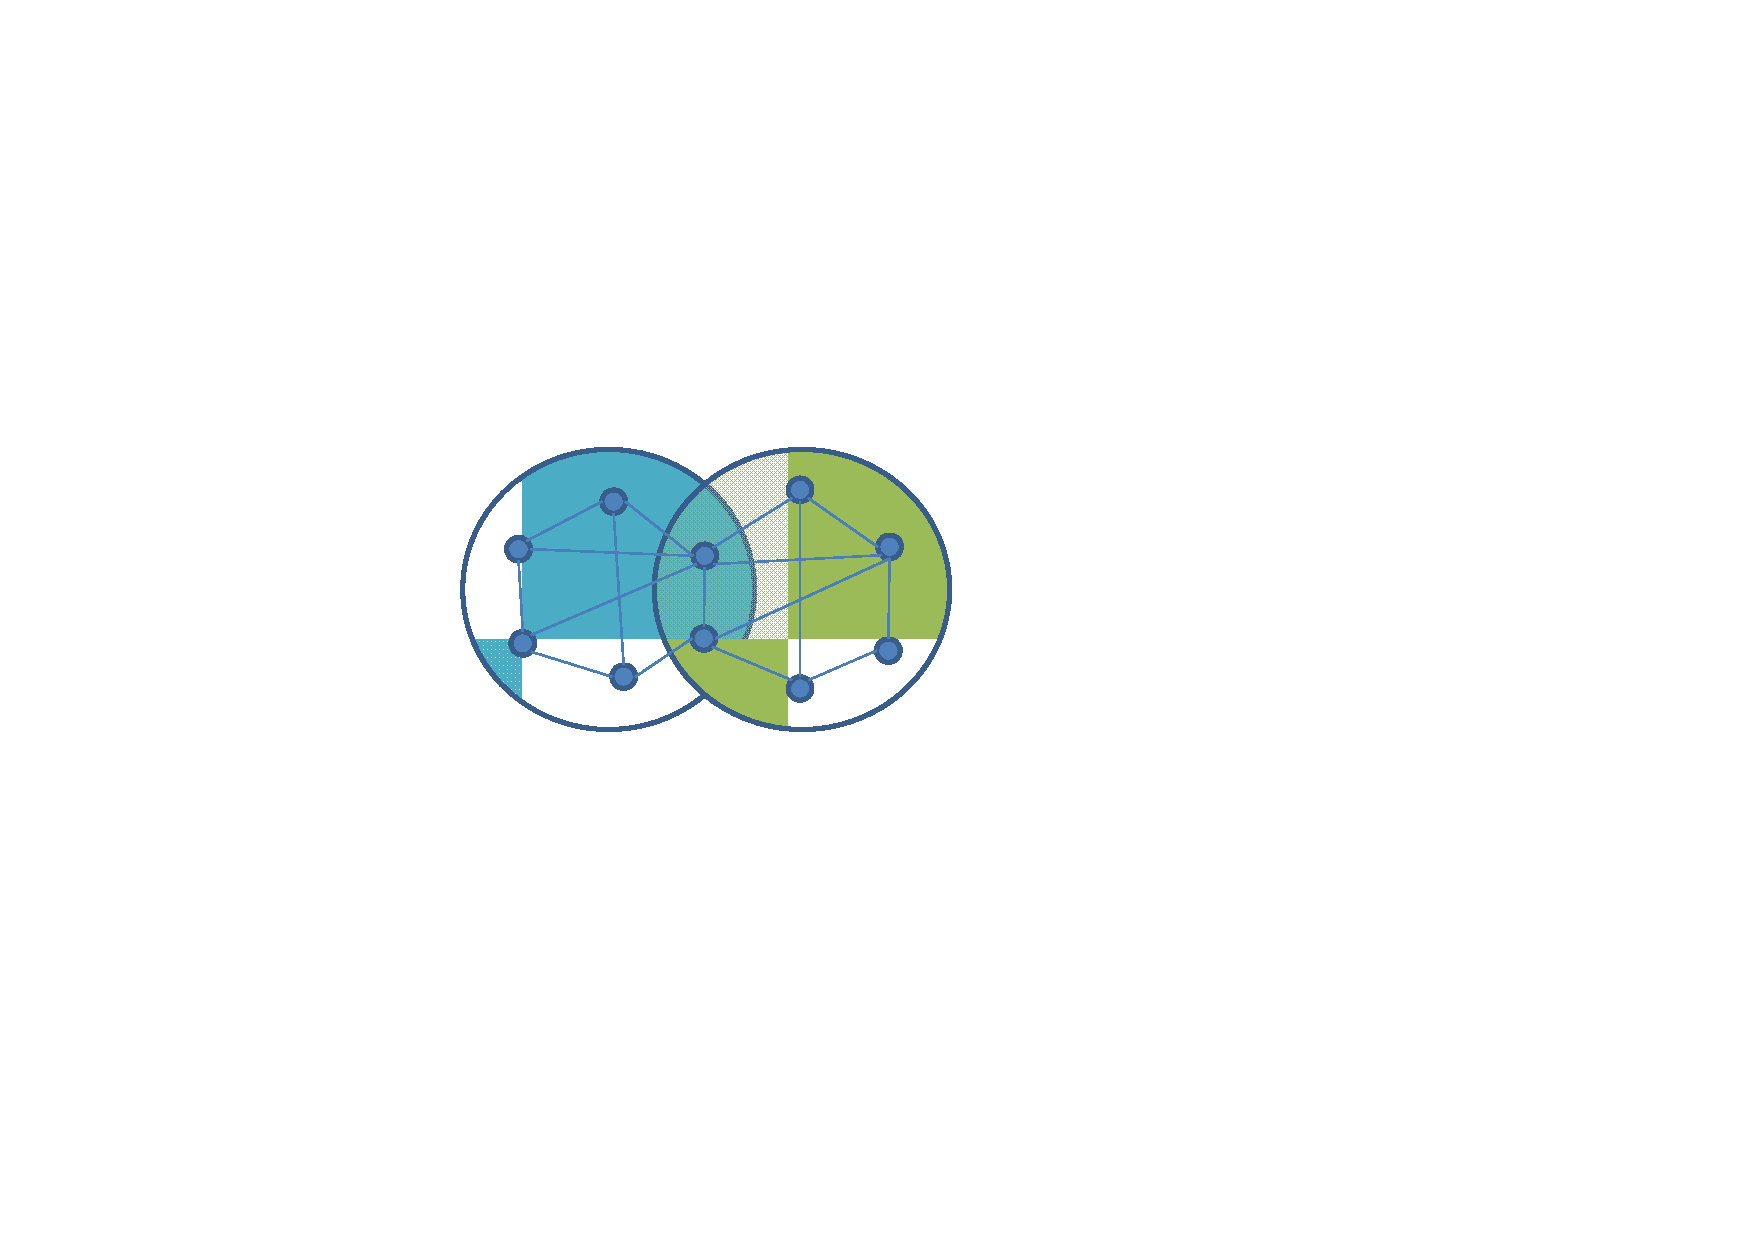
\includegraphics[height=0.14\textwidth]{figure/syn1.pdf}} &  \raisebox{-0.9\height}{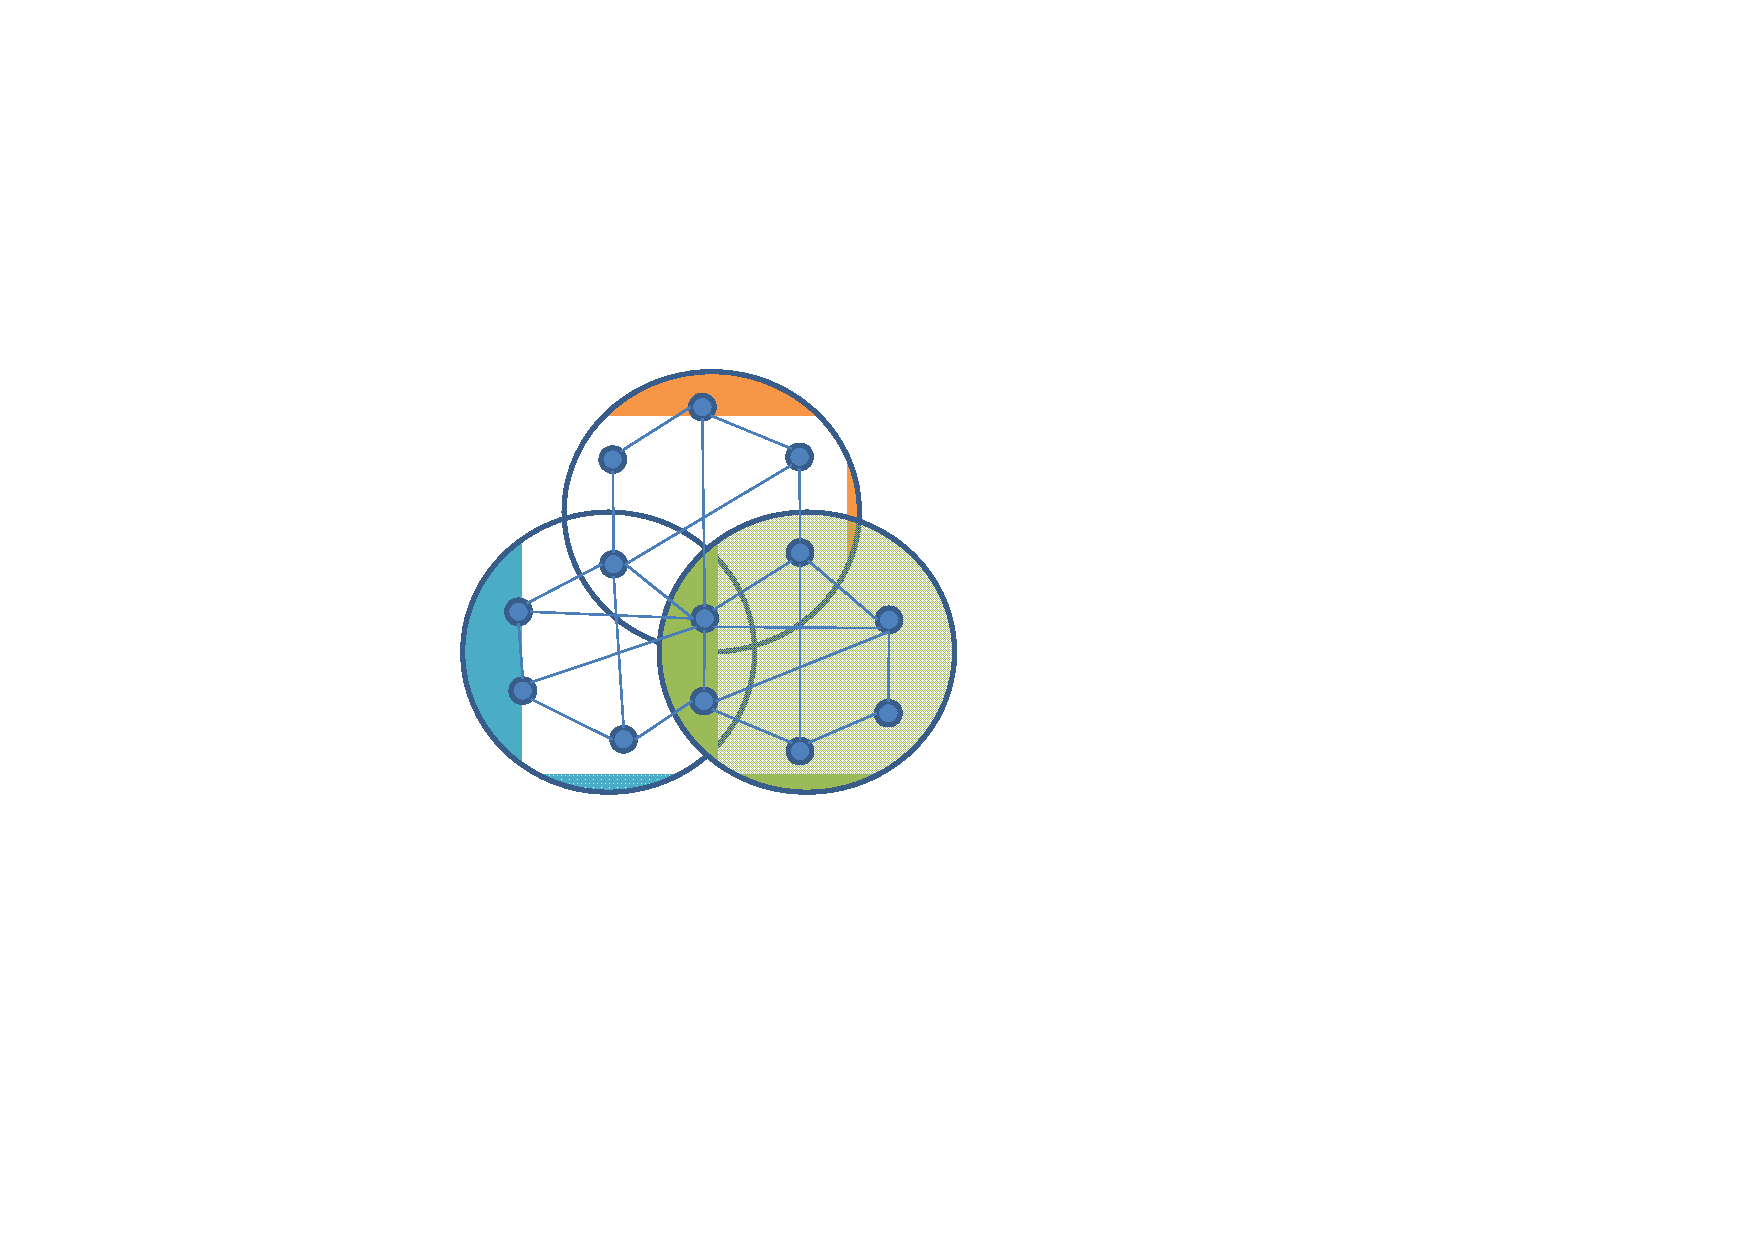
\includegraphics[height=0.14\textwidth]{figure/syn2.pdf}}  &  \raisebox{-0.9\height}{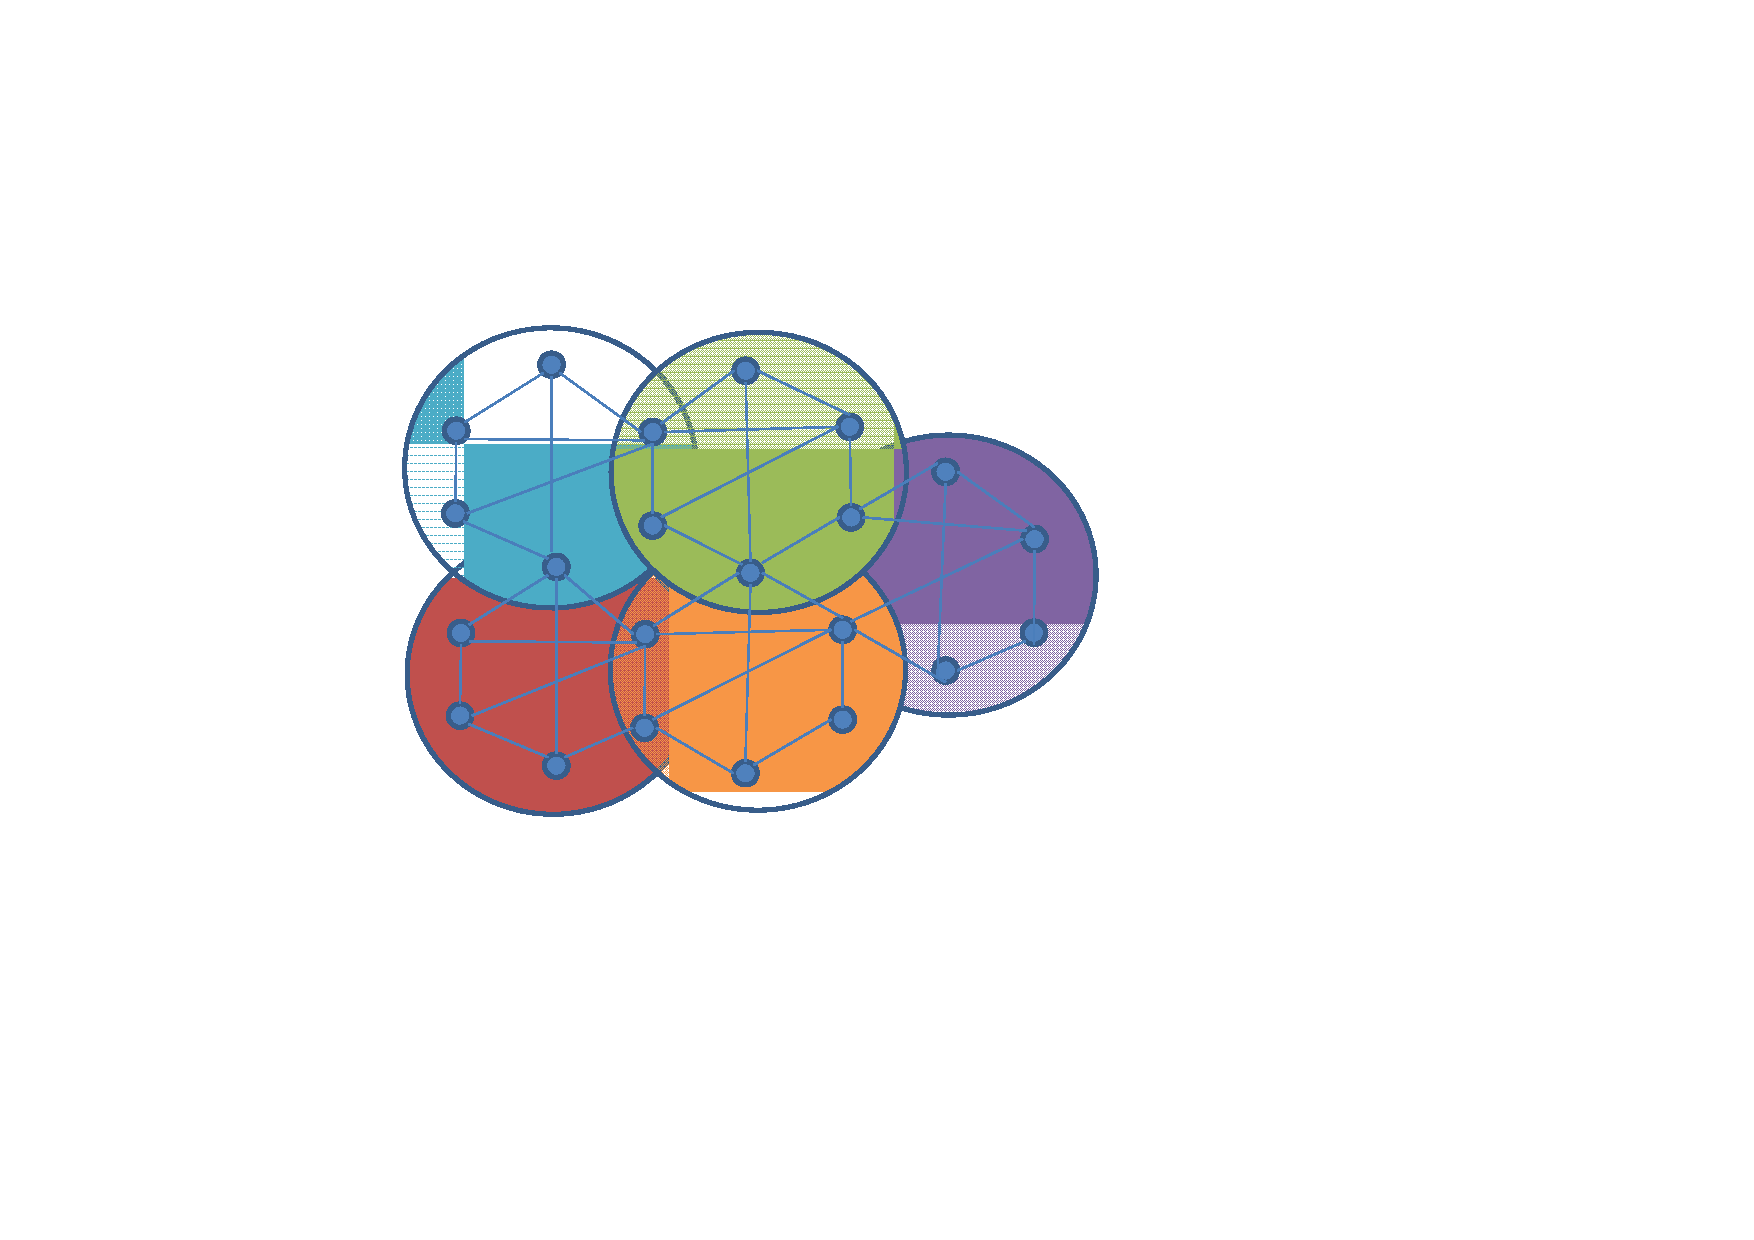
\includegraphics[height=0.14\textwidth]{figure/syn3.pdf}} \\
\hline 
Structure Setting &\tabincell{c}{$n_c = 200;n_o = 10;$\\$d_c = 0.8; d_b = 0.1$} & \tabincell{c}{$n_c = 200;n_o = 10;$\\$d_c = 0.8; d_b = 0.1$}&\tabincell{c}{$n_c = 200;n_o = 10;$\\$d_c = 0.8; d_b = 0.1$}\\
\hline
Attribute Setting&$n_d=5;n_{od}=2;r=0.05$&$n_d=8;n_{od}=2;r=0.05$&$n_d=10;n_{od}=2;r=0.05$\\
\hline
Subspace Setting& \tabincell{c}{$C1: \{1,2,...,5\}$\\$C2: \{3,4,...,8\}$ }&\tabincell{c}{$C1: \{1,2,...,8\}$\\$ C2: \{7,8,...,14\}$\\$C3: \{13,14,...,20\}$ } &\tabincell{c}{$C1: \{1,2,...,10\}$\\ $C2: \{9,10,...,18\}$\\$C3: \{17,18,...,26\}$ \\$C4: \{25,26,...,34\}$\\$C5: \{33,34,...,42\}$ }\\
\hline
%\multicolumn{4}{|c|}{\tabincell{c}{$n_c: No. vertices of each cluster; n_o: No. vertices of each overlapping; d_c: density of each cluster; d_b: density between clusters$}} \\
\end{tabular}
\label{tab:syn}
\end{table*}

%\begin{table}[t]
%\center\caption{Indexes of Generating Synthetic Attributed Graphs}
%\begin{tabular}{cc}
% \multicolumn{2}{c}{\raisebox{-0.9\height}{\includegraphics[width=0.45\textwidth]{figure/1.pdf}}} \\
% \raisebox{-0.9\height}{\includegraphics[height=0.25\textwidth]{figure/datasize.pdf}} &  \raisebox{-0.9\height}{\includegraphics[height=0.25\textwidth]{figure/dim.pdf}} \\
%\end{tabular}
%\label{tab:syn}
%\end{table}

\subsubsection{Evaluation of Clustering}
In this section, we evaluate IROC on three synthetic data sets and compare it to four relevant algorithms. PICS \cite{DBLP:conf/sdm/AkogluTMF12} is a compression based algorithm which clusters both vertices and binary attributes. BAGC \cite{DBLP:conf/sigmod/XuKWCC12} is a probability model based attributed graph partition method. DB-CSC \cite{DBLP:conf/pkdd/GunnemannBS11} is a density based algorithm which aims at detecting dense clusters with coherent subspace of attributes. It is designed for graph with numerical attributes,which chooses the attribute neighborhood if the distance of attributes of two vertices is smaller than a threshold $\epsilon$. The distance is defined as the maximum difference of all the attributes like $dist(x,y) = \max_{i\in\{1,...,T\} } |x[i]-y[i]|$. We integerize the categorical attributes of our synthetic data for DB-CSC and set $\epsilon < 1$, which means the attribute neighbors with exactly same category will be chosen. CONGO is an overlapping community detection method without considering node attributes which is adopted to compare the ability of detecting overlapping communities in structural part. Due to the multiple clustering assignments, we adopt F1-Measure to evaluate these algorithms on clustering vertices. F1-Measure is computed as the harmonic mean of Precision and Recall. Precision measures the accuracy of the detected clusters and Recall measures whether all clusters are detected.

\begin{table*}[t]
\center\caption{Evaluation Overlapping Clusters of Synthetic Data Sets}
\begin{tabular}{|c|c|c|c|c|c|c|c|c|c|}
\hline
\multirow{2}{*}{Algorithms}	& \multicolumn{3}{|c|}{Syn1} & \multicolumn{3}{|c|}{Syn2} & \multicolumn{3}{|c|}{Syn3} \\
\cline{2-10} 
      & Precision & Recall & F-Measure& Precision & Recall & F-Measure& Precision & Recall & F-Measure\\
\hline     
 IROC & \textbf{1} &\textbf{1} & \textbf{1}  & \textbf{1} & \textbf{0.973}& \textbf{0.986} & \textbf{1}& \textbf{0.963} & \textbf{0.981} \\
\hline
 PICS & 1 & 0.322 & 0.487 & 1 & 0.732& 0.846 & 0.563 & 0.670& 0.612\\
\hline
 DB-CSC &  0.895 & 0.826& 0.859 &$-$&$-$& $-$ & $-$&$-$ &$-$  \\
\hline
 BAGC &  1 & 0.947 & 0.973 & 0.955 & 0.607& 0.742 & 0.490 & 0.722& 0.584\\
\hline
 CONGO &  0.524 & 1 & 0.688 & 0.392 & 1& 0.563 &$-$&$-$ &$-$ \\
\hline 
\end{tabular}
\label{tab:fmeasuresyn}
\end{table*}

%\begin{table}[t]
%\center\caption{ The Output of Number of Clusters}
%\begin{tabular}{|c|c|c|c|c|c|c|c|}
%\hline
%Data sets & True & IROC  & PICS & DB-CSC & BAGC & DEMON\\
%\hline
%$Syn1$& 2 & 2 & 3  & 12 & 2 & 1 \\
%\hline
%$Syn2$& 3 & 3 & 3 & 23 & 3 & 6\\
%\hline
%$Syn3$& 5 & 5 & 10 & 26 & 5 & 12 \\
%\hline
%\end{tabular}
%\label{tab:clusnum}
%\end{table}

From Tab. \ref{tab:fmeasuresyn}, it is obvious that our proposed algorithm IROC outperforms the other algorithms. Generally, PICS and BAGC are not able to detect overlapping parts of graphs. DB-CSC outputs many small clusters with several overlapping vertices. However $6$ parameters have to be set. CONGO performs worse than IROC as well, which provides redundant results. Besides, it needs the number of clusters and the depth of local betweenness. Specifically, in $Syn1$ IROC achieves perfect $2$ clusters without any parameters, as shown in Fig. {\ref{fig:IROCsyn}}. From Fig. {\ref{fig:picssyn}}, parameter-free algorithm PICS outputs $8$ clusters, which splits two big cluster to several small ones. BAGC achieves $2$ clusters, which cannot detect overlapping part. DB-CSC outputs $19$ clusters and some clusters contain less than ten vertices. We run DB-CSC with $\epsilon=0.5$, $k_{min}=4$, $min_{pts}=5$,$r_{obj}=0.1$,$r_{dim}=0.1$ and $s_{min}=1$. For CONGO, we set the number of clusters to $2$ and the depth of local betweenness $h=2$. It detects a very large overlap between two clusters, which is far away from the truth. For $Syn2$, overlap exists among all the three clusters. The number of dimensions of each cluster is increased to $8$. IROC achieves $3$ perfect clusters. It also successfully detects the vertices which are assigned to all three clusters. PICS outputs $6$ clusters of vertices without overlapping. BAGC produces $3$ cluster. DB-CSC achieves no result after adjusting $6$ parameters several times and running the algorithm several days. The reason might be that DB-CSC is not applicable for dense graph with higher dimensional attributes. CONGO outputs $3$ clusters with very large overlapping parameterized with $h = 2$. $Syn3$ is more complex than the two synthetic data sets before. Similarly, IROC output $5$ good clusters. PICS partitions vertices to $7$ clusters. BAGC partitions vertices to $5$ clusters. DB-CSC still cannot output any results after increasing the number of dimension of each cluster to $10$. Due to the increased size of the data, CONGO can not achieve any results after several days running. 

\subsubsection{Evaluation of Subspace}
CONGO is designed for general graphs without node attributes and BAGC is not able to detect subspaces of attributes. PICS is an algorithm which aims at clustering the binary attributes and not at finding attributed subspaces of certain clusters. For example, Fig.\ref{fig:subspace} shows the attributed matrix of $Syn1$ after running IROC and PICS. Specifically, the size of the attributed matrix of IROC is $380 \times 8 $, where black points mean that the attribute is included in a subspace of a cluster. Two black blocks represent the clustering results of our IROC, which clearly shows the subspace of attributes and both overlaps on vertices and attributes. While the size of the attribute matrix of IROC is $380 \times 35 $. Black points mean that the vertices have corresponding categories and red lines demonstrate there are $5$ attributes clusters. It is difficult to judge which attributed clusters are part of subspace to represent the meaning of the cluster. In addition, subspaces of various clusters may contain overlap, while the clustering of attributes is not able to achieve overlaps. Besides, it is hard to obtain the binary image of DB-CSC due to the fact that too many clusters with subspace are produced. Therefore, we compare IROC with DB-CSC by evaluating F1-Measure of subspaces. Obviously, IROC achieves perfect results on every synthetic data set. The F1-Measure of DB-CSC on $Syn1$ is $0.13$, as there are many small clusters and the clustering results on structural part does not lead to detect accurate subspace. Besides, PICS obtain $10$ attributes clusters on $Syn2$ and $9$ attributes clusters on $Syn3$. Similarly, they provide no information of which attributed clusters are part of subspace to represent the meaning of the cluster.
 %
%\begin{figure}[h]
%\centering
%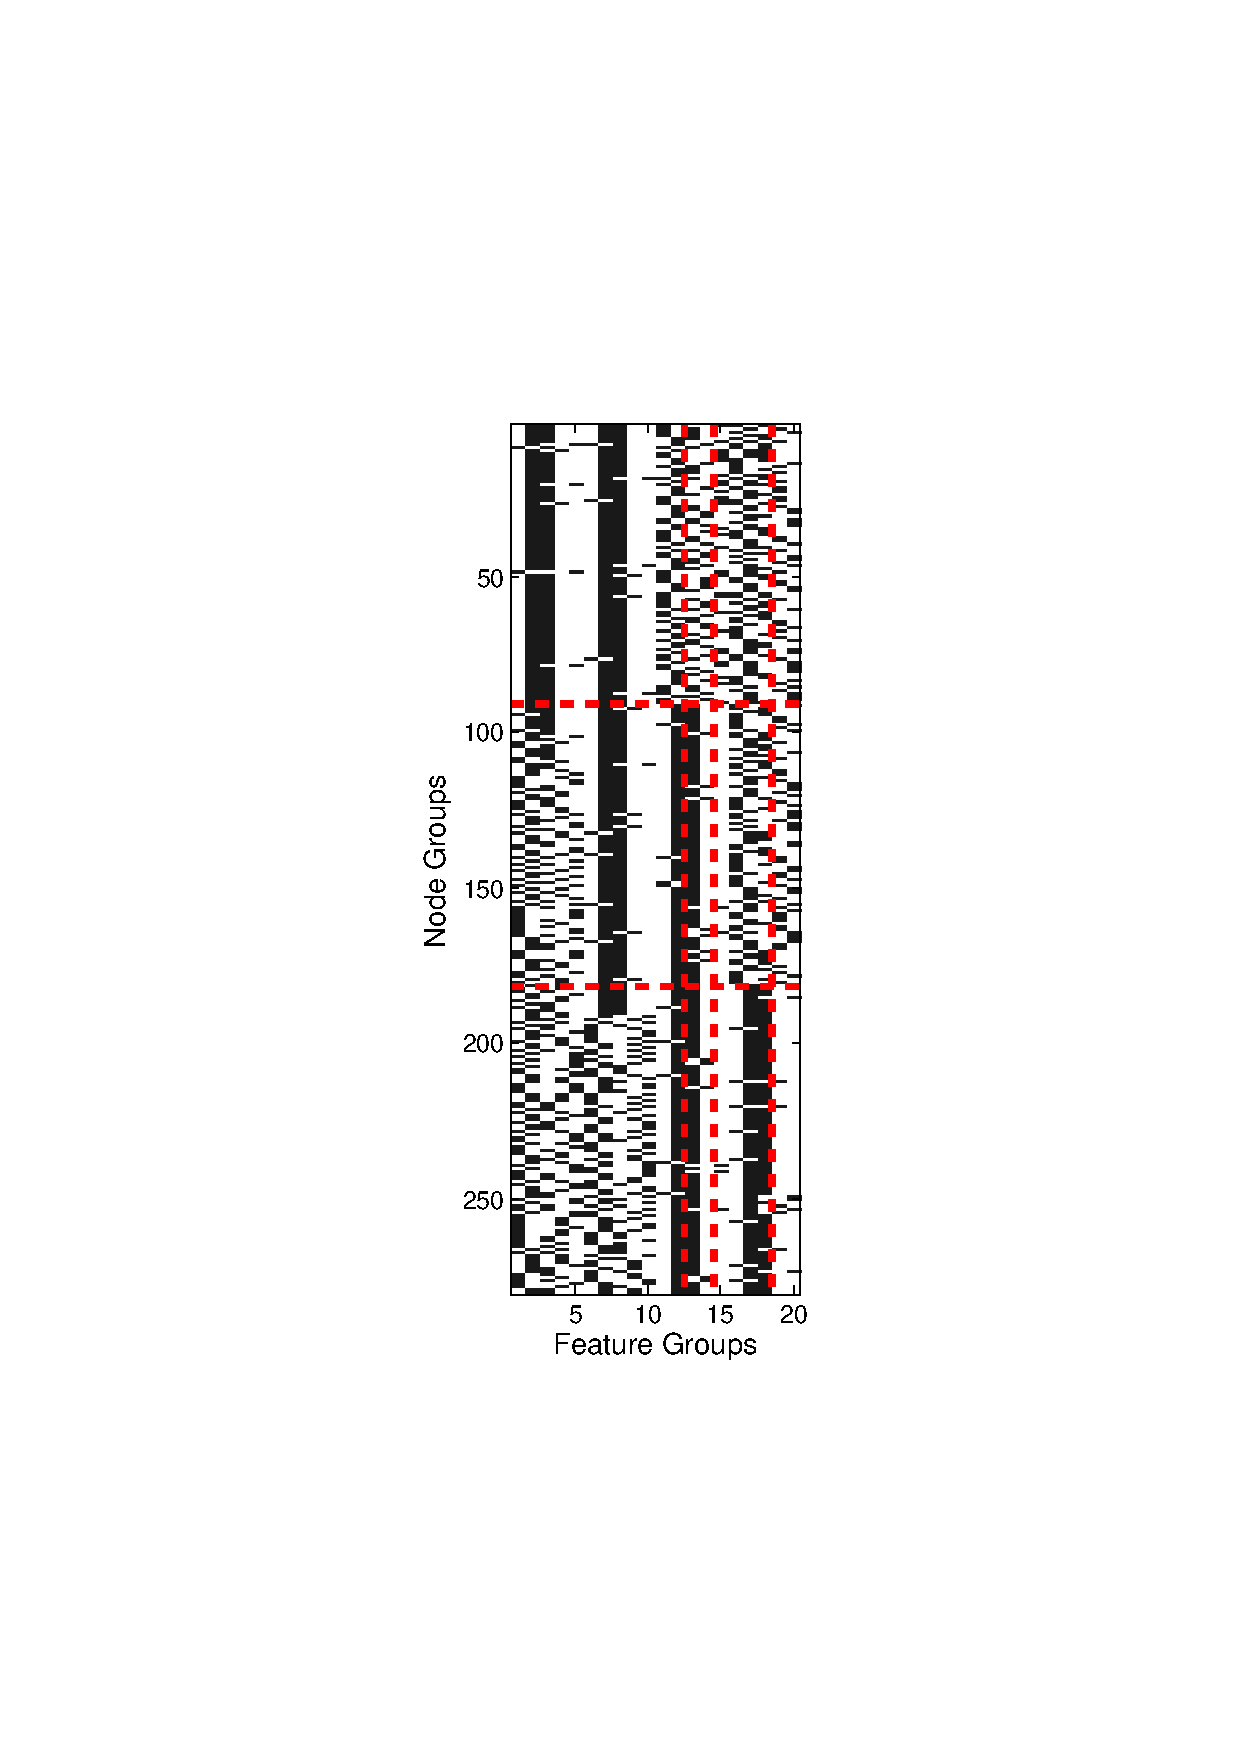
\includegraphics[height=0.8\columnwidth]{figure/3clusterPICS.pdf}
%\vspace{-3mm}
%\caption{Attribute Clustering of PICS on Syn2.}
%\label{fig:picssyn}
%\end{figure}

\begin{figure}	
	\centering
	\begin{subfigure}[h]{1.5in}
		\centering
		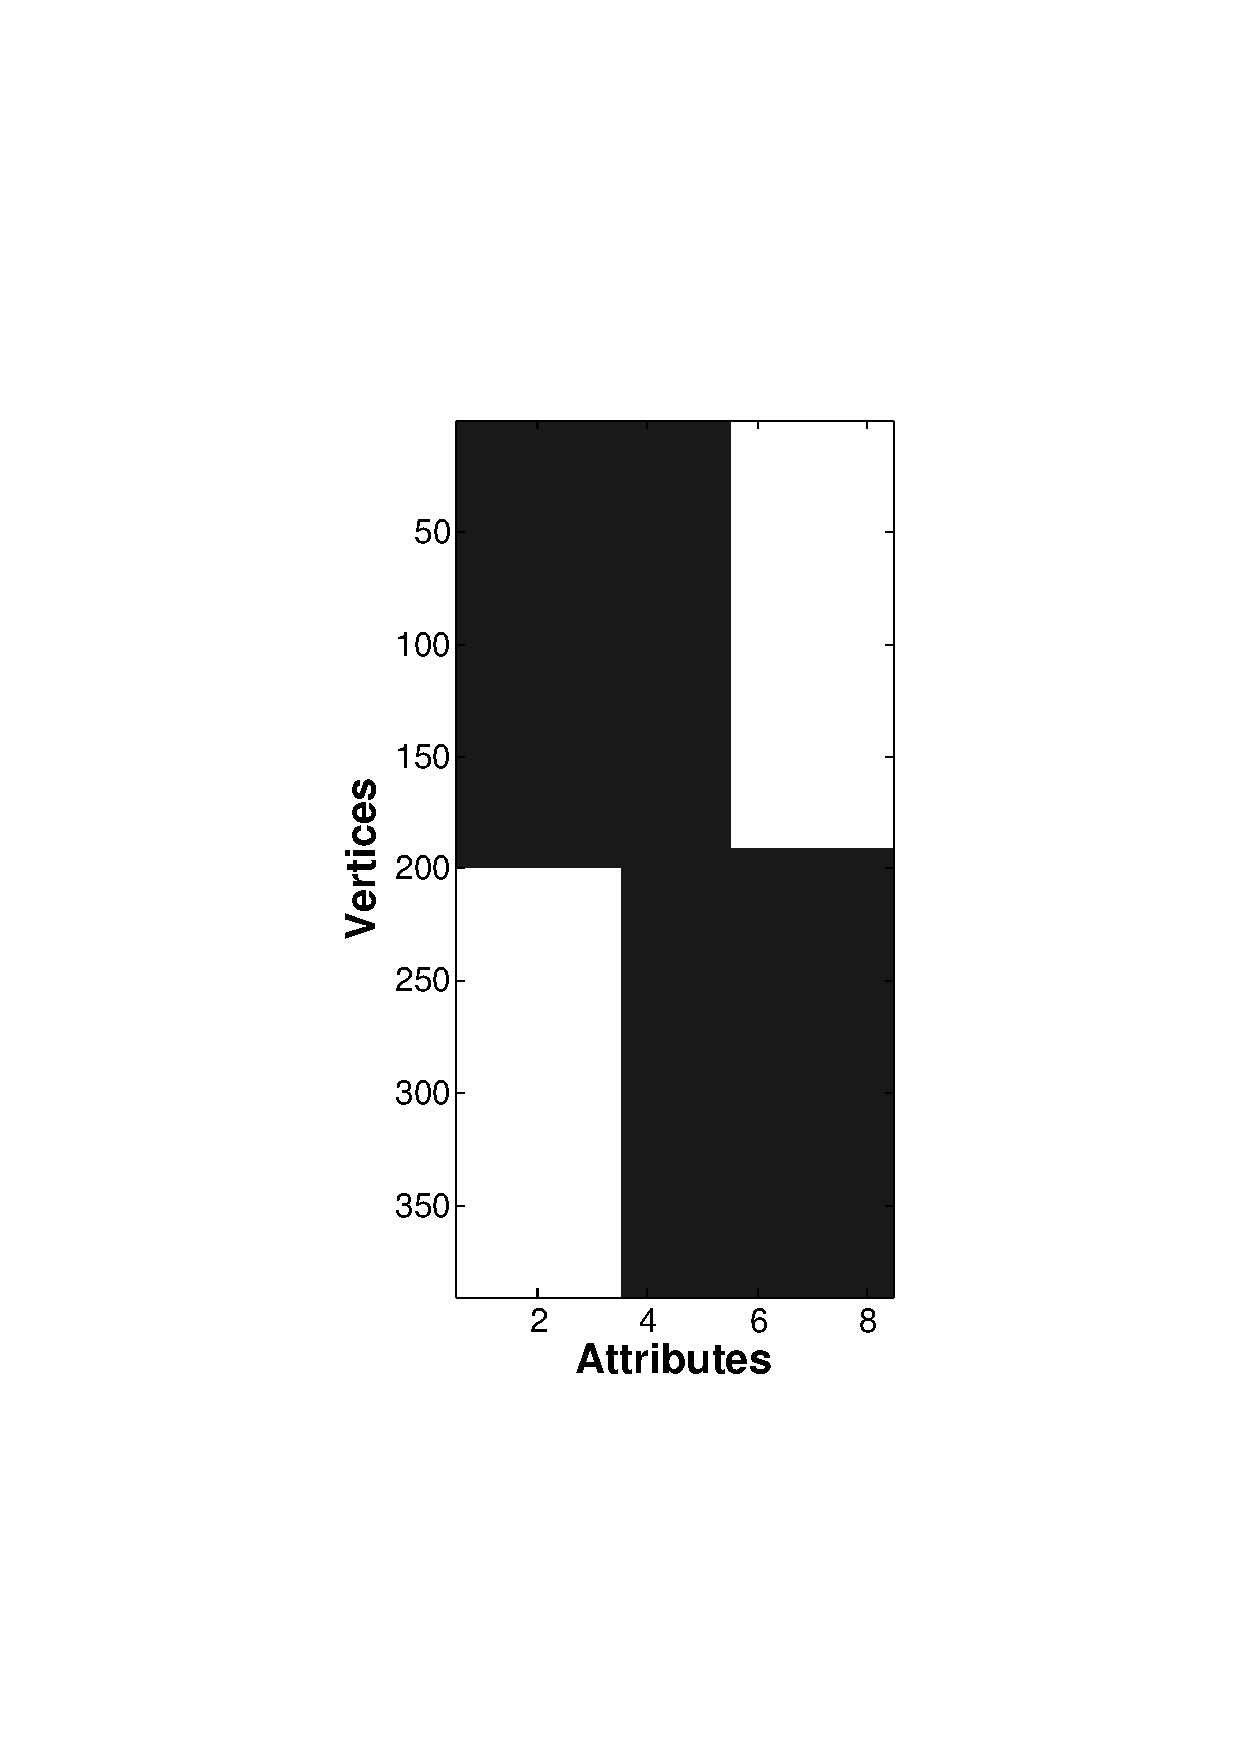
\includegraphics[height=2in]{figure/featurestander.pdf}
		\caption{IROC.}\label{fig:IROCsyn}		
	\end{subfigure}
	\quad
	\begin{subfigure}[h]{1.5in}
		\centering
		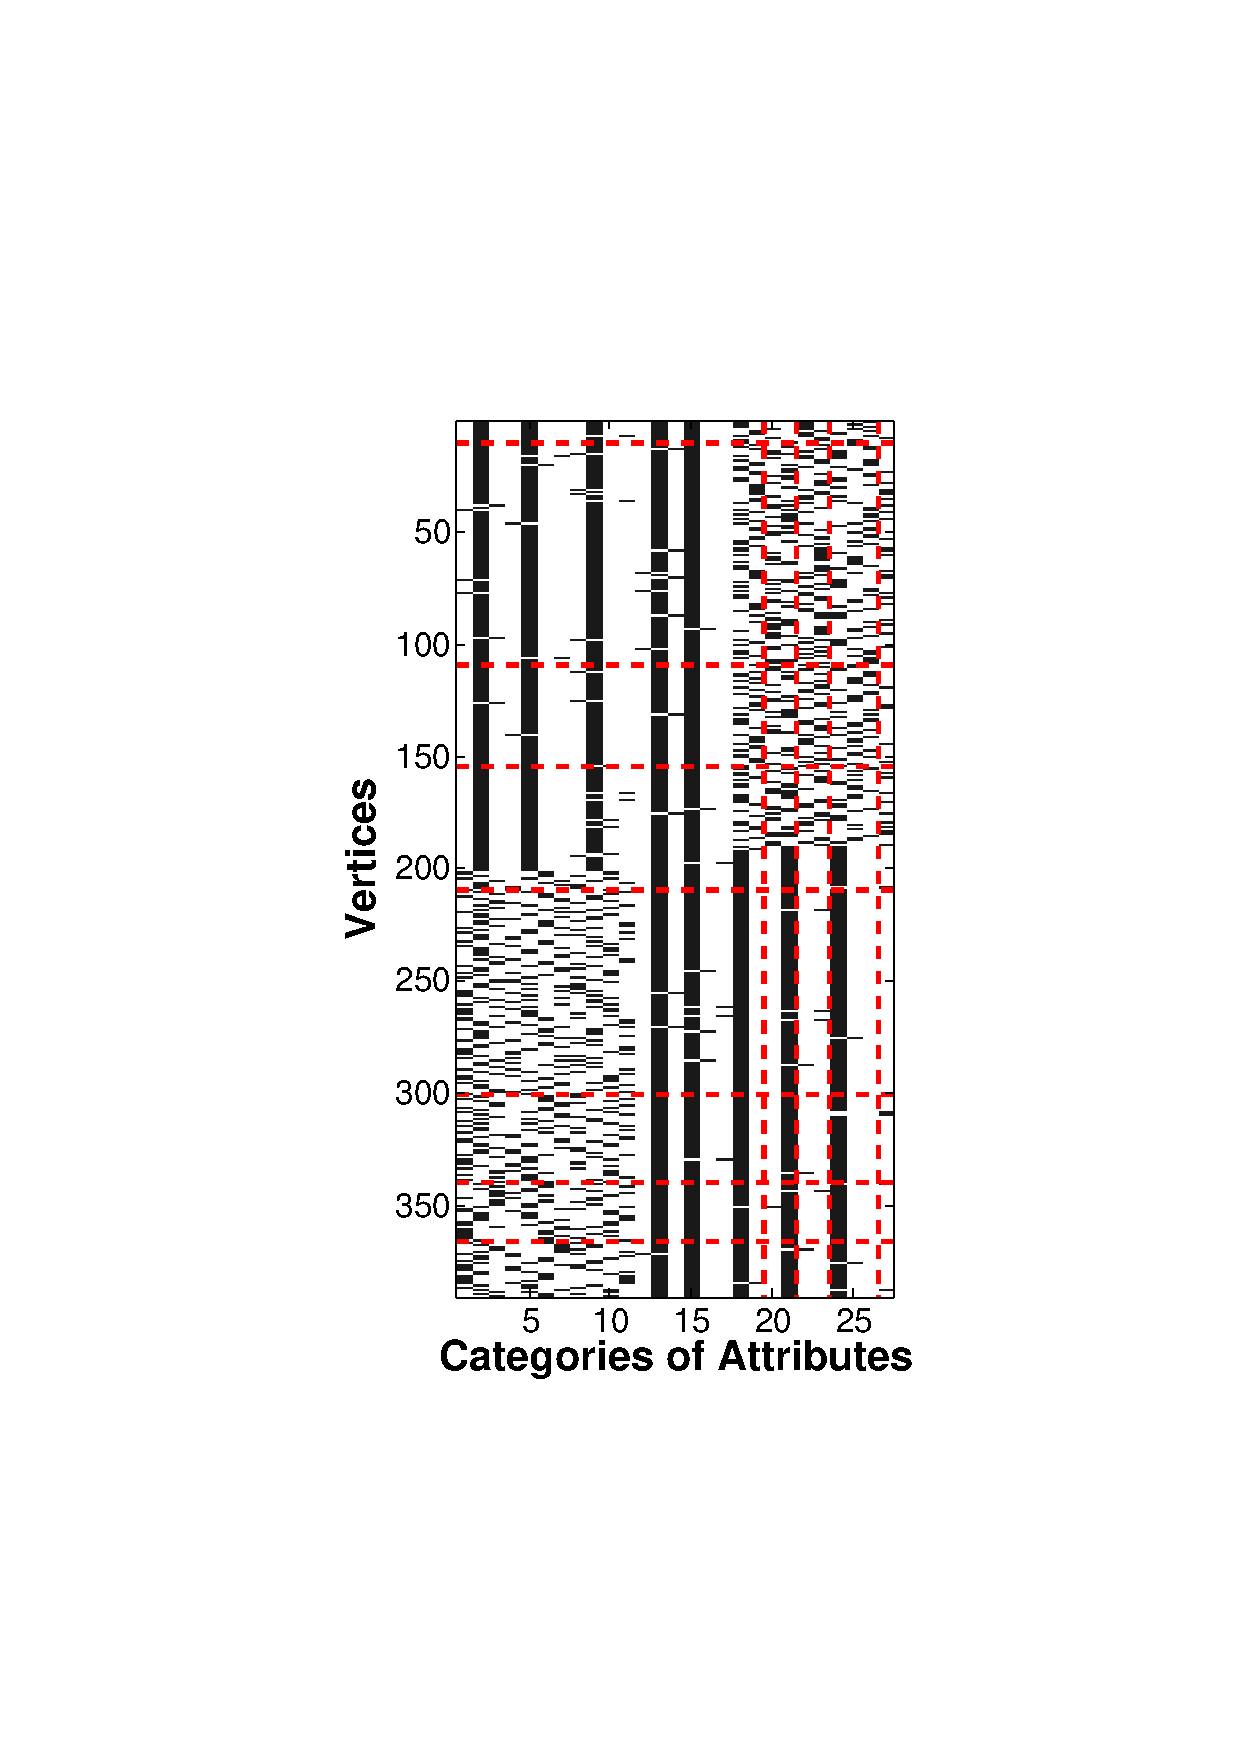
\includegraphics[height=2in]{figure/featurepics.pdf}
		\caption{PICS.}\label{fig:picssyn}
	\end{subfigure}
	\caption{Clustering Results of Syn1 in Attributed Matrix.}
	\label{fig:subspace}
\end{figure}


%\begin{table}[h]
%\center\caption{F1-Measure of Subspace}
%\begin{tabular}{|c|c|c|c|}
%\hline
%& Syn1 & Syn2 & Syn3 \\
%\hline
%$DocAG$& 1 & 1 & 1\\
%\hline
%$DB-CSC$& 0.333 & 0.155 & 0.090\\
%\hline
%\end{tabular}
%\label{tab:fmeasuresynsubspace}
%\end{table}
\subsection{Real Data sets}
\subsubsection{Facebook Data}
Facebook data sets are obtained from SNAP data sets \cite{DBLP:conf/nips/McAuleyL12}. Specifically, each Facebook data set is an ego-network of a selected node. For example, a network named $``1912"$ is generated by a node with id $1912$ and all its neighbors. Characters of vertices include birthday, education information, language, hometown, work information .etc. Each kind of property contains several anonymity items. The original node attributes are in binary form, and every single item is considered as an attribute. The value $``1"$ stands for the node that contains this item information and value $``0"$ vise verse. In this paper, we consider each type of property as attribute and the items in each property are defined as categories. In this section, we test two data sets: Ego-network $``1912"$ and Ego-network $``107"$. For the same reason with $Syn3$, we are not able to get the results from DB-CSC and CONGO after running the experiments for several days. Each data set is separated into several ``circles", but not all the vertices are included. That means only part of the vertices' label are available, thus we still use F1-Measure to compare the algorithms: IROC, PICS and BAGC. 

There are $755$ vertices in ego-network $``1912"$, and each vertex has $22$ attributes. Each attribute contains several categories, for example, there are $22$ categories in attribute "birthday" and $19$ categories in "education classes". The data set has already been labeled as $46$ circles. Obviously, Tab. \ref{tab:fmeasure1912} demonstrates that our proposed method achieves the best F1-Measure value by generating $12$ clusters. PICS generates $8$ clusters. The result of BAGC is acquired by setting the number of clusters to $46$, which equals to the given number of clusters. Ego-network $``107"$ contains $1045$ vertices, $23$ attributes and $9$ circles. Tab. \ref{tab:fmeasure1912} demonstrates that our proposed method IROC achieves the best F1-Measure value by generating $17$ clusters. PICS partitions vertices into $15$ clusters, and the result of BAGC is acquired by setting the number of clusters as $9$. Therefore, Tab.  \ref{tab:fmeasure1912} demonstrates that IROC has a big advantage in detecting vertex clusters.

\begin{table}[t]
\center\caption{F1-Measure of Facebook Data Sets }
\begin{tabular}{|c|c|c|c|c|c|}
\hline
Data sets & IROC  & PICS & BAGC \\
\hline
$Ego-network "1912"$& \textbf{0.231} & 0.224 & 0.229\\
\hline
$Ego-network "107"$& \textbf{0.141} & 0.101 & 0.118\\
\hline
\end{tabular}
\label{tab:fmeasure1912}
\end{table}

In addition, IROC discovers overlapping vertices between pairs of clusters. Take the Ego-network $``1912"$ data as an example, the analysis of overlapping is shown in Tab. \ref{tab:overlapping}. Specifically, Fig. \ref{fig:overlapping} shows a diagram of the overlapping part between cluster $C_2$ and cluster $C_{11}$. There are four overlapping vertices $``1941"$, $``2347"$, $``2468"$ and $``2543"$ forming a clique. Other vertices in $C_2$ and $C_{11}$ are both closely connected to the clique. Therefore, the two clusters $C_2$ and $C_{11}$ share the information of overlapping part and it is reasonable to assign overlapping vertices to both clusters.
\begin{table}[h]
\center\caption{Overlapping of Ego-network $"1912"$}
\small
\begin{tabular}{|c|l|}
\hline
Cluster ID & Overlapping Clusters ID(No.Vertices)\\
\hline
$C_1$ & $C_5$(1)\\
\hline
$C_2$ & \tabincell{c}{$C_3$(1), $C_4$(4), $C_5$(23), $C_6$(11), $C_7$(1), \\$C_8$(3), $C_9$(2), $C_{10}$(6) ,$C_{11}$(4), $C_{12}$(9)}\\
\hline
$C_3$ & $C_6$(1),$C_{11}$(15), $C_{12}$(4)\\
\hline
$C_4$ & $C_5$(1), $C_6$(1), $C_{11}$(11), $C_{12}$(12)\\
\hline
$C_5$ & $C_6$(1), $C_7$(1), $C_9$(1), $C_{12}$(3)\\
\hline
$C_6$ & $C_{10}$(1), $C_{12}$(3)\\
\hline
$C_{10}$ & $C_{11}$(1)\\
\hline
\end{tabular}
%\begin{tabular}{|c|c|}
%\hline
%Cluster ID & No.Overlapping \\
%\hline
%$C_1 \bigcap C_5$ & 1\\
%\hline
%$C_2 \bigcap C_3$ & 1\\
%\hline
%$C_2 \bigcap C_4$ & 4\\
%\hline
%$C_2 \bigcap C_5$ & 23\\
%\hline
%$C_2 \bigcap C_6$ & 11\\
%\hline
%$C_2 \bigcap C_7$ & 1 \\
%\hline
%$C_2 \bigcap C_8$ & 3\\
%\hline
%$C_2 \bigcap C_9$ & 2\\
%\hline
%$C_2 \bigcap C_{10}$ & 6\\
%\hline
%$C_2 \bigcap C_{11}$ & 4\\
%\hline
%$C_2 \bigcap C_{12}$ & 9\\
%\hline
%$C_3 \bigcap C_6$ & 1 \\
%\hline
%$C_3 \bigcap C_{11}$ & 15\\
%\hline
%$C_3 \bigcap C_{12}$ & 4\\
%\hline
%$C_4 \bigcap C_5$ & 1\\
%\hline
%$C_4 \bigcap C_6$ & 1\\
%\hline
%$C_4 \bigcap C_{11}$ & 1\\
%\hline
%$C_4 \bigcap C_{12}$ & 1\\
%\hline
%$C_5 \bigcap C_6$ & 1\\
%\hline
%$C_5 \bigcap C_7$ & 1\\
%\hline
%$C_5 \bigcap C_9$ & 1\\
%\hline
%$C_5 \bigcap C_{12}$ & 3\\
%\hline
%$C_6 \bigcap C_{10}$ & 1\\
%\hline
%$C_6 \bigcap C_{12}$ & 3\\
%\hline
%$C_{10} \bigcap C_{11}$ & 1\\
%\hline
%\end{tabular}
\label{tab:overlapping}
\end{table}

\begin{figure}[h]
\centering
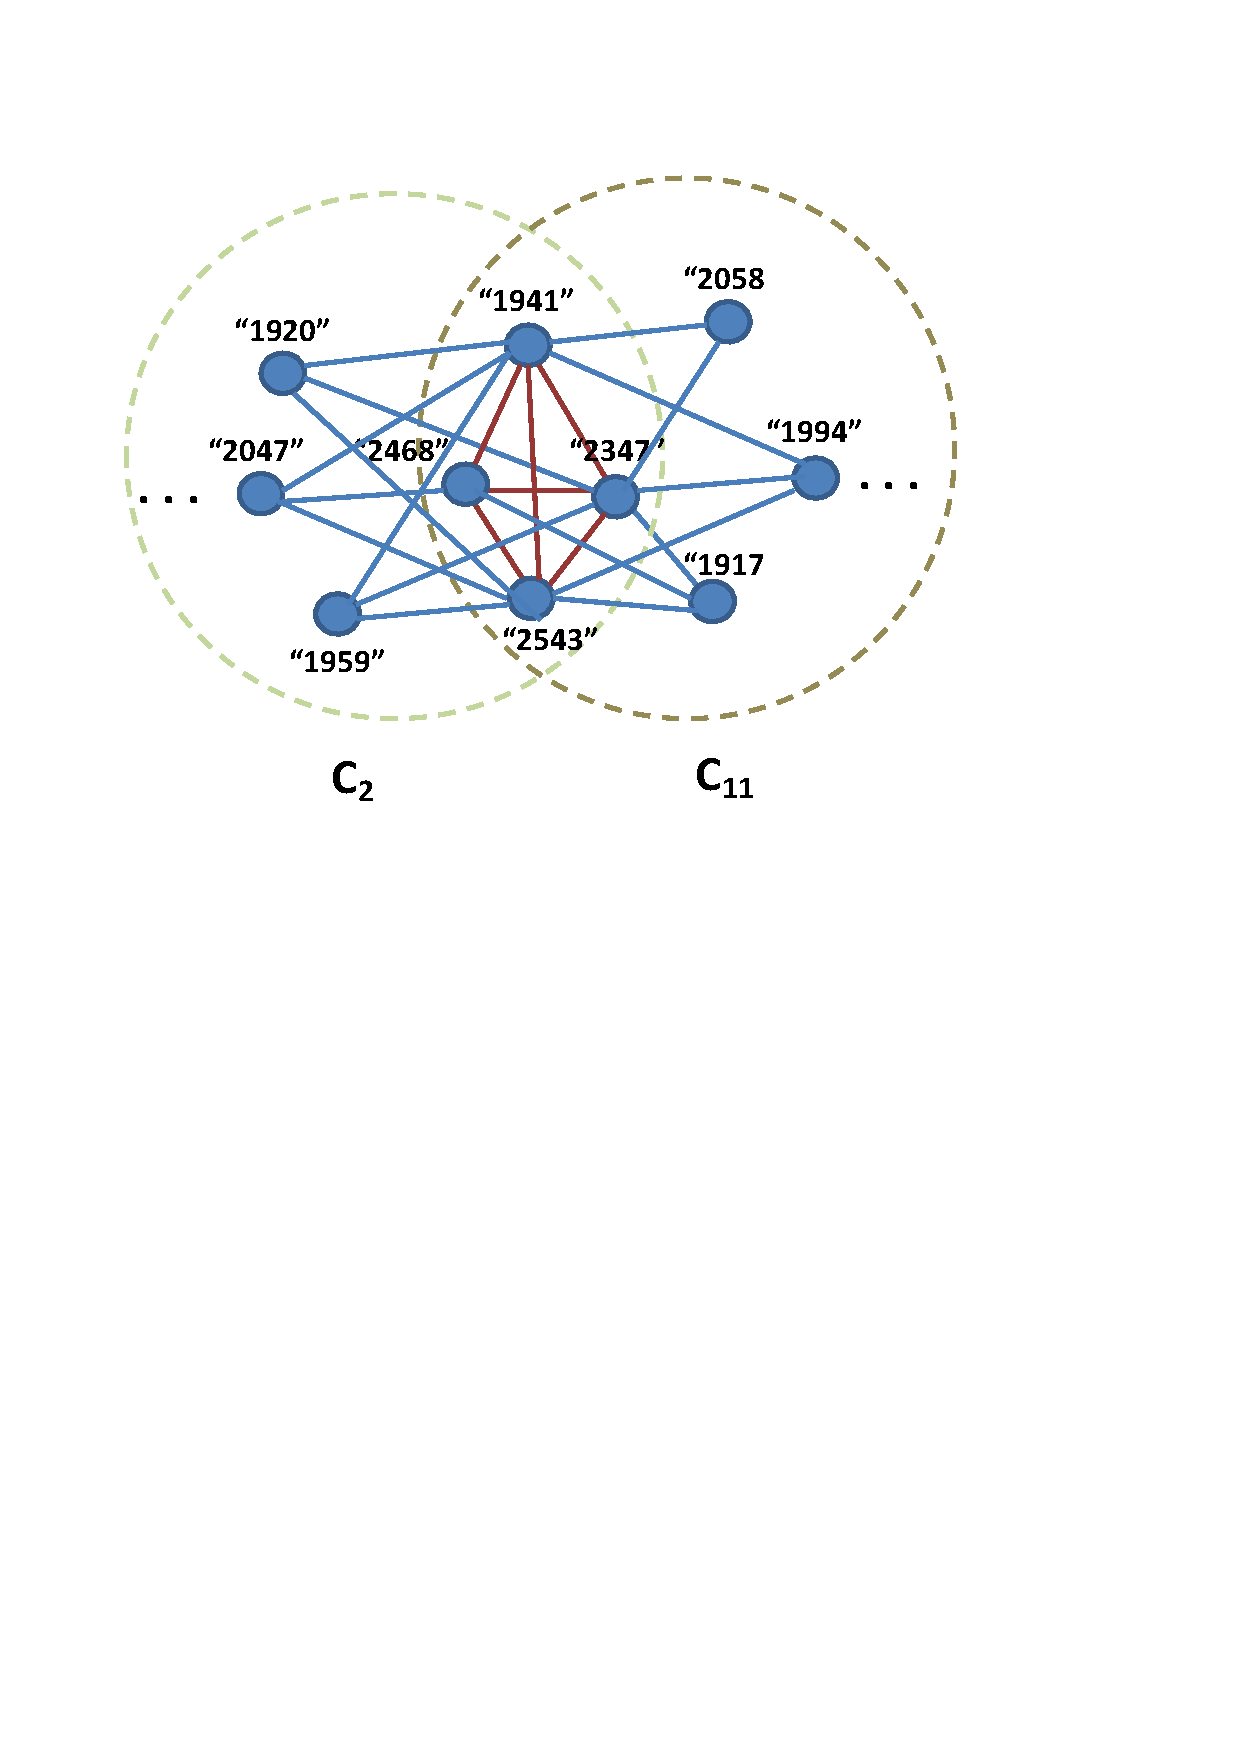
\includegraphics[width = 0.6\columnwidth]{figure/graph.pdf}
\vspace{-3mm}
\caption{Overlapping Between Cluster $2$ and Cluster $11$ of Ego-network "1912".}
\label{fig:overlapping}
\end{figure}

Betweenness centrality of a vertex is the ratio of the number of the shortest paths from $v_m$ to $v_n$ through vertex $v$ to the number of all shortest paths from $v_m$ to $v_n$ which is shown in Eq. (\ref{eq:betweenness}).
\begin{equation}
Betweeness(v)= \sum_{v_m\neq v\neq v_n}\frac{Path_{v_mv_n}(v)}{Path_{v_mv_n}}.
\label{eq:betweenness}
\end{equation}
Where betweenness centrality measures the ability of a human communicating with other humans in a social network \cite{betweeness}. That is to say, vertex with high betweenness plays the role of bridge. We calculate betweenness centrality of all the vertices, and rank them in descending order. Take the overlapping part of $C_2$ and $C_{11}$ as an example, the rank of the betweenness values of $``1941"$, $``2347"$, $``2468"$ and $``2543"$ is $5$, $4$, $20$ and $3$ separately, which possesses really high betweenness centrality values. Then these four persons are very outgoing and sociable. They communicate with various communities, so that they are assigned to multiple clusters. Besides, the betweenness values of all overlapping vertices are large, which implies that these vertices possess higher ability to communicate with other vertices thus assigning into multiple clusters.


%\begin{table}[h]
%\center\caption{Top 10 vertex Ranking by Betweeness Centrality}
%%\begin{tabular}{|c|c|c|c|c|c|c|c|c|c|}
%%\hline
%%Vertex ID & Rank & Vertex ID & Rank & Vertex ID & Rank & Vertex ID & Rank & Vertex ID & Rank &\\
%%\hline
%%"3497"& 24 & "3539" & 72 & "3632" & 5 & "3943" & 76 & "3504" & 143\\
%%\hline
%%"3761"& 20 & "3833" & 280 & "3971" & 91 & "3440" & 133 & "3522" & 4\\
%%\hline
%%"3559"& 131 & "3608" & 2 & "3666" & 148 & "3835" & 1 & "3896" & 101\\
%%\hline
%%"3934"& 271 & "3935" & 56 & "3590" & 79 & "3682" & 34 & "3507" & 75\\
%%\hline
%%"3561"& 174 & "3588" & 51 & "3597" & 93 & "3685" & 7 & "3763" & 82\\
%%\hline
%%"3798"& 42 & "3905" & 200 & "3911" & 71 & "3952" & 226 & "3556" & 94\\
%%\hline
%%"3710"& 6 & "3442" & 15 & "3633" & 87 & \\
%%\hline
%%\end{tabular}
%\begin{tabular}{|c|c|c|c|}
%\hline
%Rank & Vertex ID & Rank & Vertex ID \\
%\hline
%1 & \textbf{"3835"} & 6 & \textbf{"3710"}\\
%\hline
%2 & \textbf{"3608"} & 7 & \textbf{"3685"} \\
%\hline
%3 & "3923" & 8 & "3569"\\
%\hline
%4 & \textbf{"3522"} & 9 & "3621"\\
%\hline
%5 & \textbf{"3632"} & 10 & "3785" \\
%\hline
%\end{tabular}
%\label{tab:rank3437}
%\end{table}

Regarding the attributes, BAGC is not able to detect any subspace of clusters. PICS detects $8$ attributes clusters in Ego-network $``1912"$ and $11$ attributes clusters in Ego-network $``107"$. Our IROC detects a subspace of attributes for each cluster. Tab. \ref{tab:subspace1912} shows the attributes subspaces of Ego-network $``1912"$. The table shows that overlaps also exist between subspaces. For example, $C_5$ and $C_6$ have one vertex overlapping, and meanwhile their subspaces also overlap on attribute "middle name".

\begin{table}[h]
\center\caption{Subspace detected by IROC  of Ego-network $"1912"$}
\small
\begin{tabular}{|c|c|}
\hline
Cluster ID & Subspace\\
\hline
$C_1$ & all 22 attributes\\
\hline
$C_2$ & "middle name"\\
\hline
$C_3$ & "middle name","work projects"\\
\hline
$C_4$ & all 22 attributes\\
\hline
$C_5$ & "middle name","work projects"\\
\hline
$C_6$ & "middle name"\\
\hline
$C_7$ & all 22 attributes\\
\hline
$C_8$ & all 22 attributes\\
\hline
$C_9$ & all 22 attributes\\
\hline
$C_{10}$ & "work projects"\\
\hline
$C_{11}$ & "work projects"\\
\hline
$C_{12}$ & "middle name"\\
\hline
\end{tabular}
\label{tab:subspace1912}
\end{table}

%\begin{figure}[h]
%\centering
%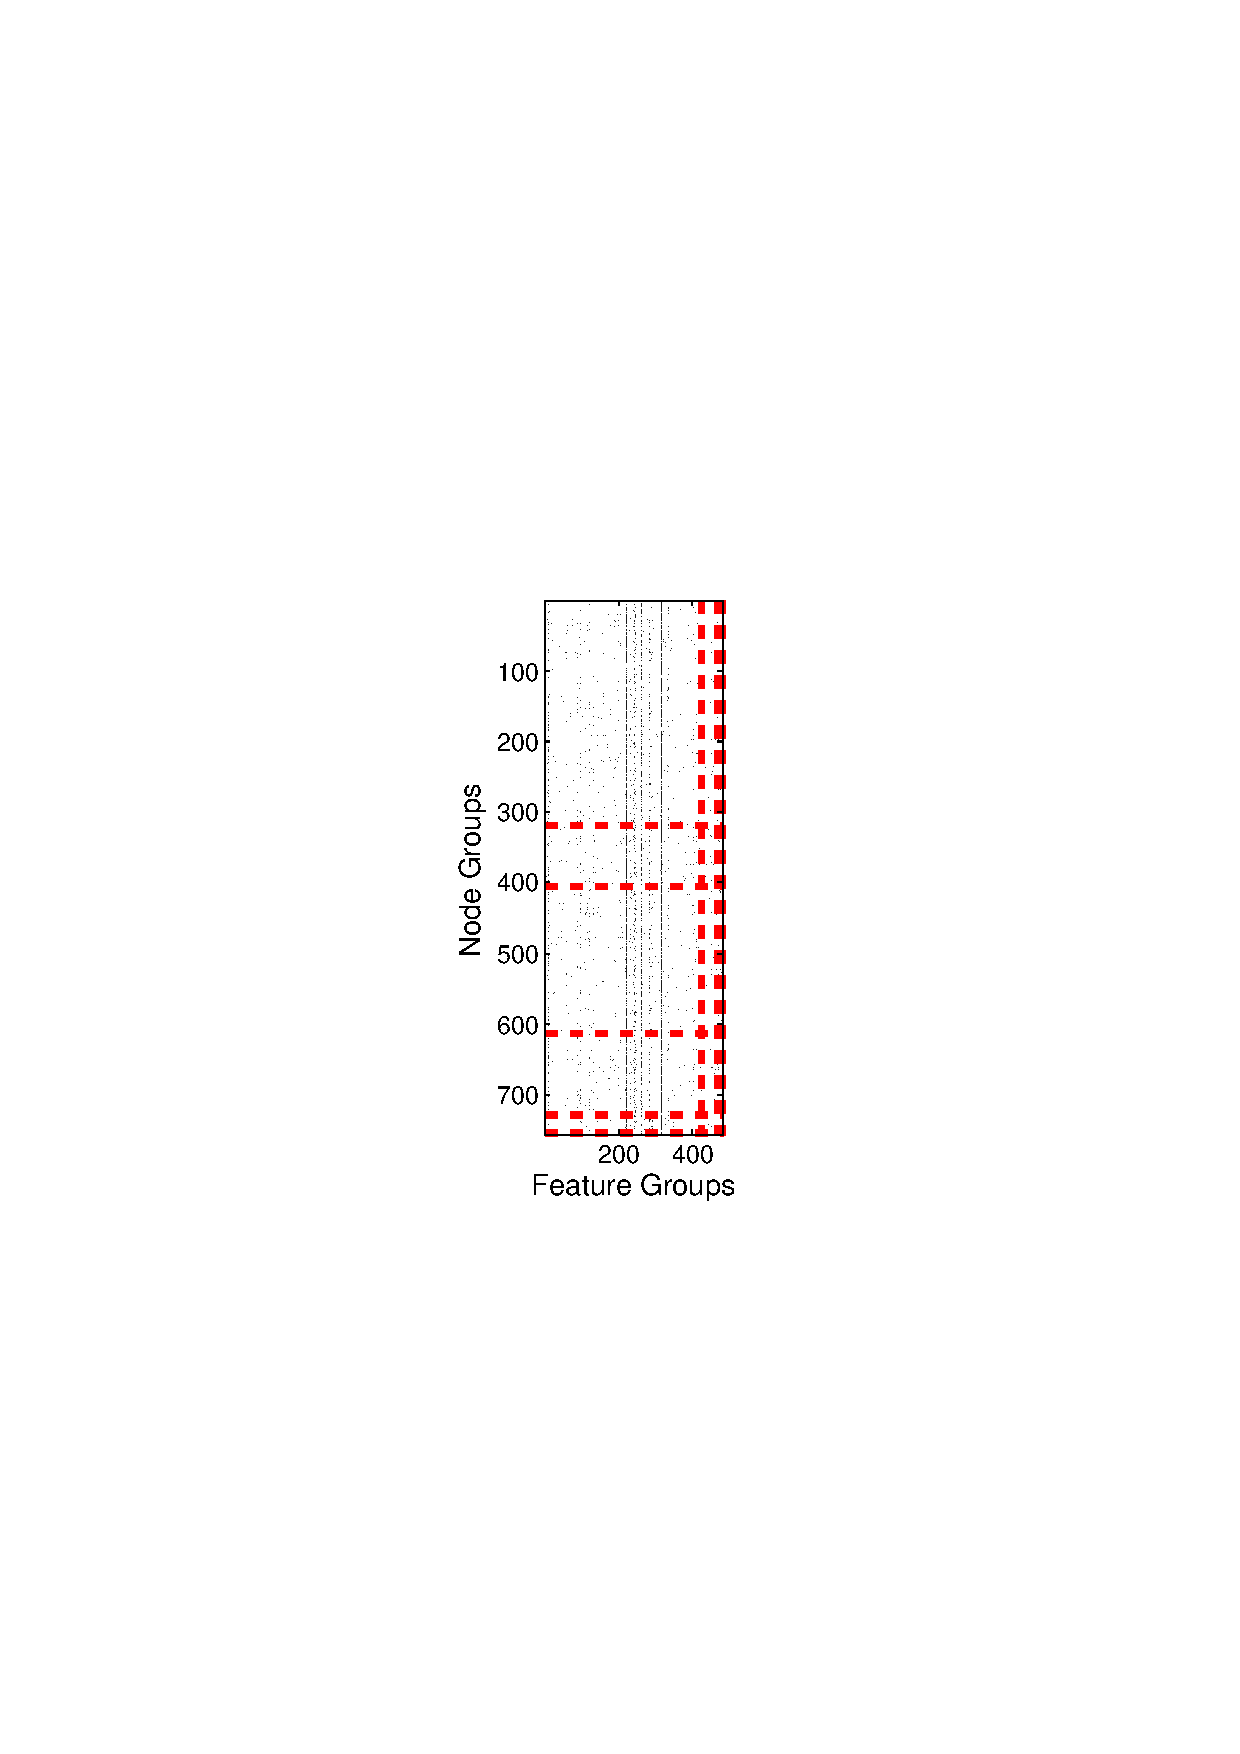
\includegraphics[height=0.5\columnwidth]{figure/PICS1912.pdf}
%\vspace{-3mm}
%\caption{Attribute Clustering of PICS on Ego-network "1912".}
%\label{fig:pics1912}
%\end{figure}


%\begin{table}[h]
%\center\caption{Subspace detected by IROC  of Ego-network $"107"$}
%\begin{tabular}{|c|c|}
%\hline
%Cluster ID & Subspace\\
%\hline
%$C_1$ & all 23 attributes\\
%\hline
%$C_2$ & all 23 attributes\\
%\hline
%$C_3$ & all 23 attributes\\
%\hline
%$C_4$ & "work with"\\
%\hline
%$C_5$ & all 23 attributes\\
%\hline
%$C_6$ & all 23 attributes\\
%\hline
%$C_7$ & all 23 attributes\\
%\hline
%$C_8$ & "middle name"\\
%\hline
%$C_9$ & all 23 attributes\\
%\hline
%$C_{10}$ & all 23 attributes\\
%\hline
%$C_{11}$ & "work from"\\
%\hline
%$C_{12}$ & "work projects"\\
%\hline
%$C_{13}$ & all 23 attributes\\
%\hline
%$C_{14}$ & "work projects"\\
%\hline
%$C_{15}$ & "education with"\\
%\hline
%$C_{16}$ & ""work from""\\
%\hline
%$C_{17}$ & all 23 attributes\\
%\hline
%\end{tabular}
%\label{tab:subspace107}
%\end{table} 
\newpage
\subsubsection{Google+ Data}
Google+ data sets are obtained from SNAP data sets \cite{DBLP:conf/nips/McAuleyL12} as well. Specifically, each Google+ data set is also an ego-network of a selected node. Similarly, we transfer the given binary feature to categorical feature which contains $6$ attributes: gender, institution, job title, last name, place and university. Similarly, part of labels are given as circles, thus we compare F1-Measure of the algorithms: IROC, PICS, BAGC and DBCSC. 

Tab. \ref{tab:fmeasuregp} shows that IROC achieves the best clustering result among all the algorithms. Take the data set $``gp53"$ which contains $1084$ vertices and $6$ attributes for example, our proposed algorithm IROC detects $17$ clusters with overlapping and without redundancy. Each cluster is provided with an attribute subspace which represents the meaning of the clusters. For example, people in one cluster are connected densely and all of them are from the same university, or people in one cluster are densely connected and all of them are from the same institution. Moreover, PICS outputs $12$ vertices clusters and $6$ attributes clusters. We set the number of cluster of BAGC to $4$, which equals to the given number of circles. DBCSC outputs $15$ clusters parametrized with $\epsilon=0.5$, $k_{min}=2$, $min_{pts}=3$,$r_{obj}=0.3$,$r_{dim}=0.3,s_{min}=3$. All the $15$ detected clusters are provided with a subspace. However, there are three clusters with exactly same vertices which contain redundant information.
\begin{table}[t]
\center\caption{F1-Measure of Google+ Data Sets }
\begin{tabular}{|c|c|c|c|c|c|}
\hline
Data sets & IROC  & PICS & BAGC & DBCSC \\
\hline
gp7 & \textbf{0.248} & 0.205 & 0.236 & 0.106\\
\hline
gp53 & \textbf{0.289} & 0.125 & 0.130& 0.074\\
\hline
\end{tabular}
\label{tab:fmeasuregp}
\end{table}
\section{Related Work and Discussion}
Our proposed algorithm IROC is design for clustering the attributed graph under the permission of overlapping in both vertices and the subspace of attributes. The related work therefore comprises two parts: attributed graph clustering and overlapping community detection methods.

\subsection{Attributed Graph Clustering}
Attributed graph is an extension of general graph by involving the attributes of the vertices. The key point of mining such complex data is to combine structural connections and characteristics of the vertices. Paper \cite{DBLP:journals/pvldb/ZhouCY09} augments graphs by considering each attribute as vertex. A Random walk is utilized on the augmented graph so as to create a unified similarity measure which combines structural and attribute information. However, the algorithm is carried out in a K-Medoids framework and partitions the attributed graph. It also needs to input the number of clusters and parameters for the random walk, such as number of steps and the probability to go back. Moreover, paper \cite{DBLP:conf/icdm/ZhouCY10} proposes an incremental algorithm to improve efficiency of \cite{DBLP:journals/pvldb/ZhouCY09}. Paper \cite{DBLP:conf/sigmod/XuKWCC12} proposes an algorithm named BAGC based on Bayesian probabilistic model to partition attributed graphs. Structural and attributed information are fused by the probabilistic model and clustering problem is transferred to a probabilistic inference problem. Similarly, the algorithm needs to input the number of clusters, and many other parameters to construct the necessary probability distribution. Obviously, these partition based methods can not detect any overlapping of clusters. And they do not find coherent attributed subspace of cluster. For these partitioning approaches, we choose BAGC as a comparison method. 

Guennemann et al. proposes an algorithm named DB-CSC (Density-Based Combined Subspace Clustering) \cite{DBLP:conf/pkdd/GunnemannBS11} which is based on the classical density-based clustering algorithm DBSCAN \cite{DBLP:conf/kdd/EsterKSX96}. The new proposed DB-CSC inherits the advantages of DBSCAN which can detect clusters of arbitrary shapes and sizes. It defines a combined local neighborhood by finding vertices, which belong to the intersects of $k$-neighborhood of vertices and $\epsilon$-neighborhood of subspace of the attributes. Based on the new defined neighborhood, some density related properties like high local density, local connected and maximality is defined, thus the fulfilled clusters can be detected. Instead of giving the number of clusters, DB-CSC needs parameters like $\epsilon$-neighborhood, $k$-neighborhood and a minimum number Minpts. In order to remove redundant clusters of the above two algorithms, the authors proposed a definition which is used to calculate redundancy between clusters. After adopting the strategy of removing redundancy clusters, the combined new algorithms need more parameters, $robj$ and $rdim$ which measure how much overlap between clusters is allowed without redundancy. Therefore, DB-CSC needs an isolate process and set several parameters to remove redundancy. If the parameters is set unpropertied, redundancy still exists. In comparison, IROC obtains the non-redundant results without setting any parameters. Moreover, as mentioned in experiments part, judging from the distance defined in the paper, DB-CSC is defined to deal with the attributed graphs with numerical attributes. But categorical attributes like gender, hobby .etc are common in social network data set. Therefore, IROC is able to detect overlapping clusters of the categorical attributed graph and meanwhile find the coherent attribute subspace of each cluster.    


%Guennemann et al. propose Gamer\cite{DBLP:conf/icdm/GunnemannFBS10} and DB-CSC\cite{DBLP:conf/pkdd/GunnemannBS11}, which combines dense subgraph mining with subspace clustering. In experimental section, we choose the latest DB-CSC as a comparison method. In DB-CSC, a new neighborhood which combines structure and attribute information is defined to fit the density based clustering implemented on graph data with additional feature vectors. Clusters with overlapping can be detected, meanwhile corresponding subspace can be discovered by depth first searching. However, density based algorithm need to predefine many parameters and many clusters are produced as well as redundancy. Most importantly, DB-CSC is restricted to some types of overlap: Within the same subspace clusters are not allowed to overlap in terms of the objects. Overlap is only possible for graph clusters in different subspaces. Our proposed algorithm combine structural and attributed information based on information theoretic ideas and is not restricted to some specific types of overlap. All possible combinations of overlap in terms of objects and subspaces are in principle possible but only reported as a result if they pay-off with respect to data compression. IROC is the first method balancing quality and redundancy in an information-theoretic way.
 
PICS\cite{DBLP:conf/sdm/AkogluTMF12} is also a parameter free algorithm based on MDL principle. It is able to mine cohesive clusters from an attributed graph with similar connectivity patterns and homogeneous attributes. However, it can not detect any overlapping and it cluster the vertices and attributes separately. Thus it is hard to find out which subspace belongs to which clusters. Additionally, Sun et al. \cite{DBLP:journals/pvldb/SunAH12} proposes a model-based method to clustering heterogeneous information networks which are containing incomplete attributes and multiple link relations. Also marginally related to our method are the approaches \cite{DBLP:journals/pvldb/SilvaMZ12}\cite{DBLP:conf/sdm/MoserCRE09}\cite{DBLP:conf/kdd/TongFGE07} achieving numerous small cohesive subgraphs, which aim to discover a correlation between node attributes and small subgraphs. Paper \cite{DBLP:conf/sigmod/TianHP08} summarizes multi-relational attributed graphs by aggregating nodes by using selected attributes and relations.

\subsection{Detecting Overlapping Communities}
The key point of acquiring overlapping clusters is how to assign a vertex to multiple labels. In first instance, \cite{nature} reveals overlapping phenomena of complex networks in nature, and achieves overlapping communities by seeking k-cliques which contains overlapping vertices. Paper \cite{DBLP:conf/kdd/ZhangY12} proposes an algorithm based on matrix factorization. The assignment of each vertices is stored as probability in a matrix with a number of dimensions equal to the number of the community. By fuzzy allocation, overlap between communities is achieved. CONGA\cite{DBLP:conf/pkdd/Gregory07} proposed by Gregory is an algorithm which aims to detect overlapping communities by iteratively calculating two betweenness centrality based concepts ``edge betweenness" and ``split betweenness" of all edges and vertices respectively and removing the edge or splitting the vertex with the highest value until no edges remain. As betweenness centrality is a global measure of vertices in a graph, the calculation of the two concepts depends on counting the number of shortest paths of all pairs of vertices, which is really time consuming. In order to speed up the algorithm CONGA, the author proposes an algorithm named CONGO\cite{DBLP:conf/pkdd/Gregory08} by calculating local betweenness instead of global betweenness. In the new algorithm, a parameter $h$ is added, which is a threshold that the shortest path which is more than h is ignored. Thus the concepts only need to recalculate locally to save time complexity. Both CONGA and CONGO need user to predetermined the number of clusters $k$. In this paper, we compare IROC with CONGO to prove the efficiency of our algorithm to detect overlapping clusters. Actually, the overlapping community detection algorithms which are mentioned above are all only considering the structural information of graph with no additional attributes.


% Gregory proposes an algorithm named CONGA\cite{DBLP:conf/pkdd/Gregory07}, which is based on measuring betweenness centrality. By continuous splitting the vertex with the highest betweenness value, the communities are formed and meanwhile the vertex is assigned to multiple communities. Then a fast algorithm\cite{DBLP:conf/pkdd/Gregory08} is proposed for speeding up CONGA by calculating a local betweenness value. Coscia et al.\cite{DBLP:conf/kdd/CosciaRGP12} proposes an algorithm by extracting redundancy subgraphs by defining graph operations, label propagation algorithm performance on these subgraphs while merging them to obtain the overlapping communities. Similarly, our algorithm is achieving its overlapping community by mining redundancy of subgraphs. However, comparing with our algorithm, this algorithm outputs too much clusters with large redundancy. 





\section{Conclusion}
Summarizing this work, we introduced the first solution that is
explicitly able to find meaningful overlapping in the graph structure
as well as in its respective attribute subspace. We outlined the importance
of these overlapping communities especially for attributed graphs and the information
gain that can be received by it.
Our method IROC applied the concept of information theoretic measures like entropy
and an Minimum Description length (MDL) formula designed for this callenge
 to elegantly avoid a) redundancy in the attribute space as well as in the network itself and
 b) the need to set in an unsupervised setting typically unknown input parameters to achieve good results.
Our experiments clearly showed that IROC is able to outperform all relevant comparison methods on synthetic data and on real world data of social networks.


\bibliographystyle{abbrv}
\bibliography{sigproc}  % sigproc.bib is the name of the Bibliography in this case

\end{document}